\section{Results}\label{sec:results}

We first discuss the choice of $k$ and the 2DPCA reconstructions, then the cross-validation results, the comparison with baselines and ablations, the tests under moonlight and clouds, and finally the SHAP maps and full-night time series.

\subsection{2DPCA Spectrum and Reconstruction Residuals}\label{sec:kselect}

To choose the number of projection vectors $k$, we looked at the eigenvalue spectrum of the image covariance matrix together with the 5-fold cross-validated F1-score on the training split for $k \in \{1, 2, 3, 5, 10, 15, 20, 25, 30\}$ (Figure~\ref{fig:2dpca_variance}).

\begin{figure}[htbp]
    \centering
    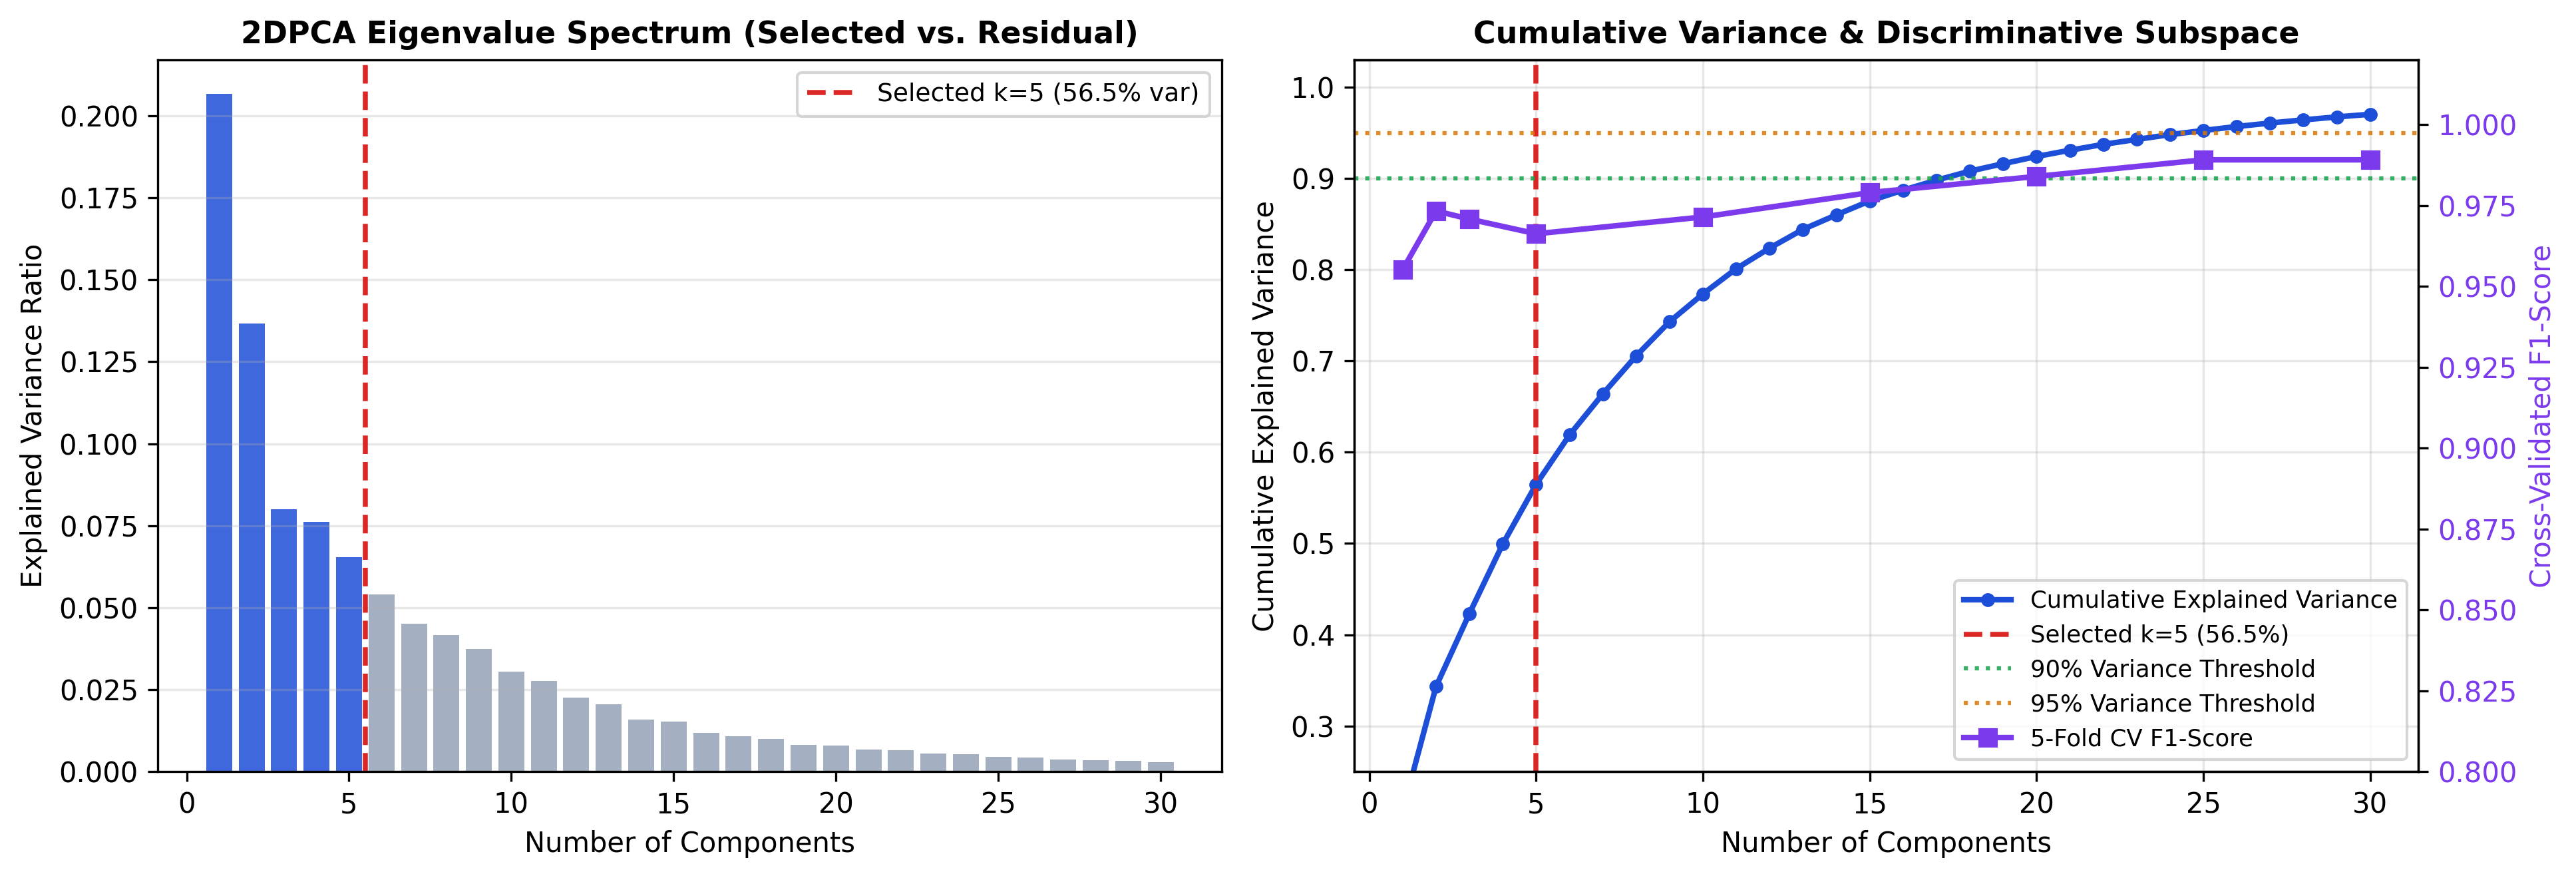
\includegraphics[width=0.98\textwidth]{figs/2dpca_variance.png}
    \caption{Left: Individual explained variance ratio across the first $30$ 2DPCA components (out of $64$) on the augmented training split, indicating the selected $k=5$ cutoff ($56.5\%$ cumulative variance). Right: Cumulative explained variance and 5-fold cross-validated F1-score from $k=1$ to $k=30$.}
    \label{fig:2dpca_variance}
\end{figure}

Since background subtraction and CLAHE are applied before the covariance is estimated, the uniform illumination mode, which accounts for nearly $80\%$ of the variance of raw images, is no longer present, and the variance spreads over more components. On the unaugmented training set ($n=429$), the cumulative variance goes from $22.86\%$ at $k=1$ to $59.41\%$ at $k=5$, $79.03\%$ at $k=10$, and $95.69\%$ at $k=25$. The components beyond $k=5$ mostly add fine-scale variance from residual stars and sensor grain, while the F1-score already exceeds $0.966$ at $k=5$. We therefore kept $k=5$ ($320$ features), which retains the mesoscale structure of the depletions and avoids the $1600\text{--}1920$ features required at $k=25\text{--}30$, a large number for a few hundred training images.

\begin{figure}[htbp]
    \centering
    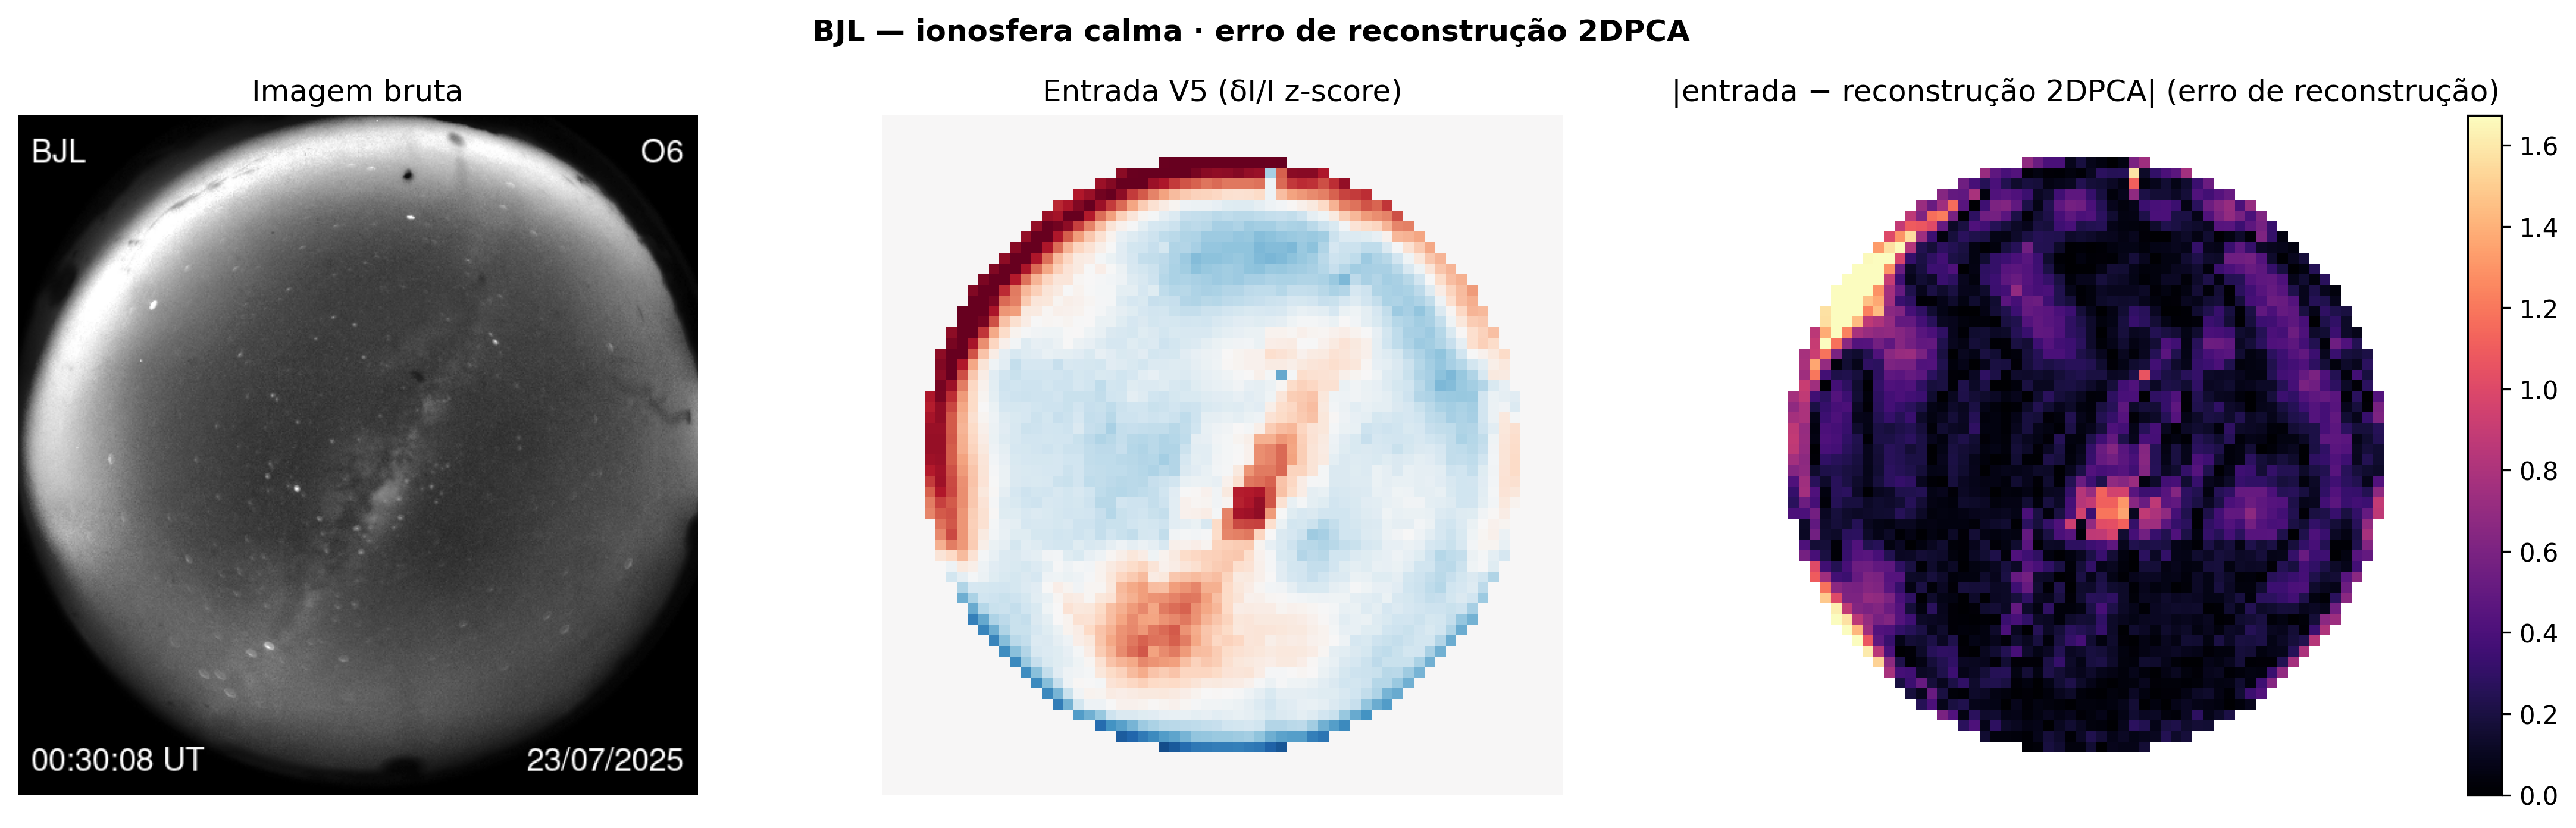
\includegraphics[width=0.96\textwidth]{figs/recon_error_without.png}
    \caption{Unsupervised 2DPCA subspace reconstruction analysis for a quiet-sky exposure (No EPB, predicted EPB probability $0.4\%$). Left: raw $630.0\text{ nm}$ image. Center: preprocessed $64 \times 64$ matrix $\mathbf{X}$. Right: reconstruction residual $|\mathbf{X} - \hat{\mathbf{X}}|$.}
    \label{fig:recon_error_without}
\end{figure}

\begin{figure}[htbp]
    \centering
    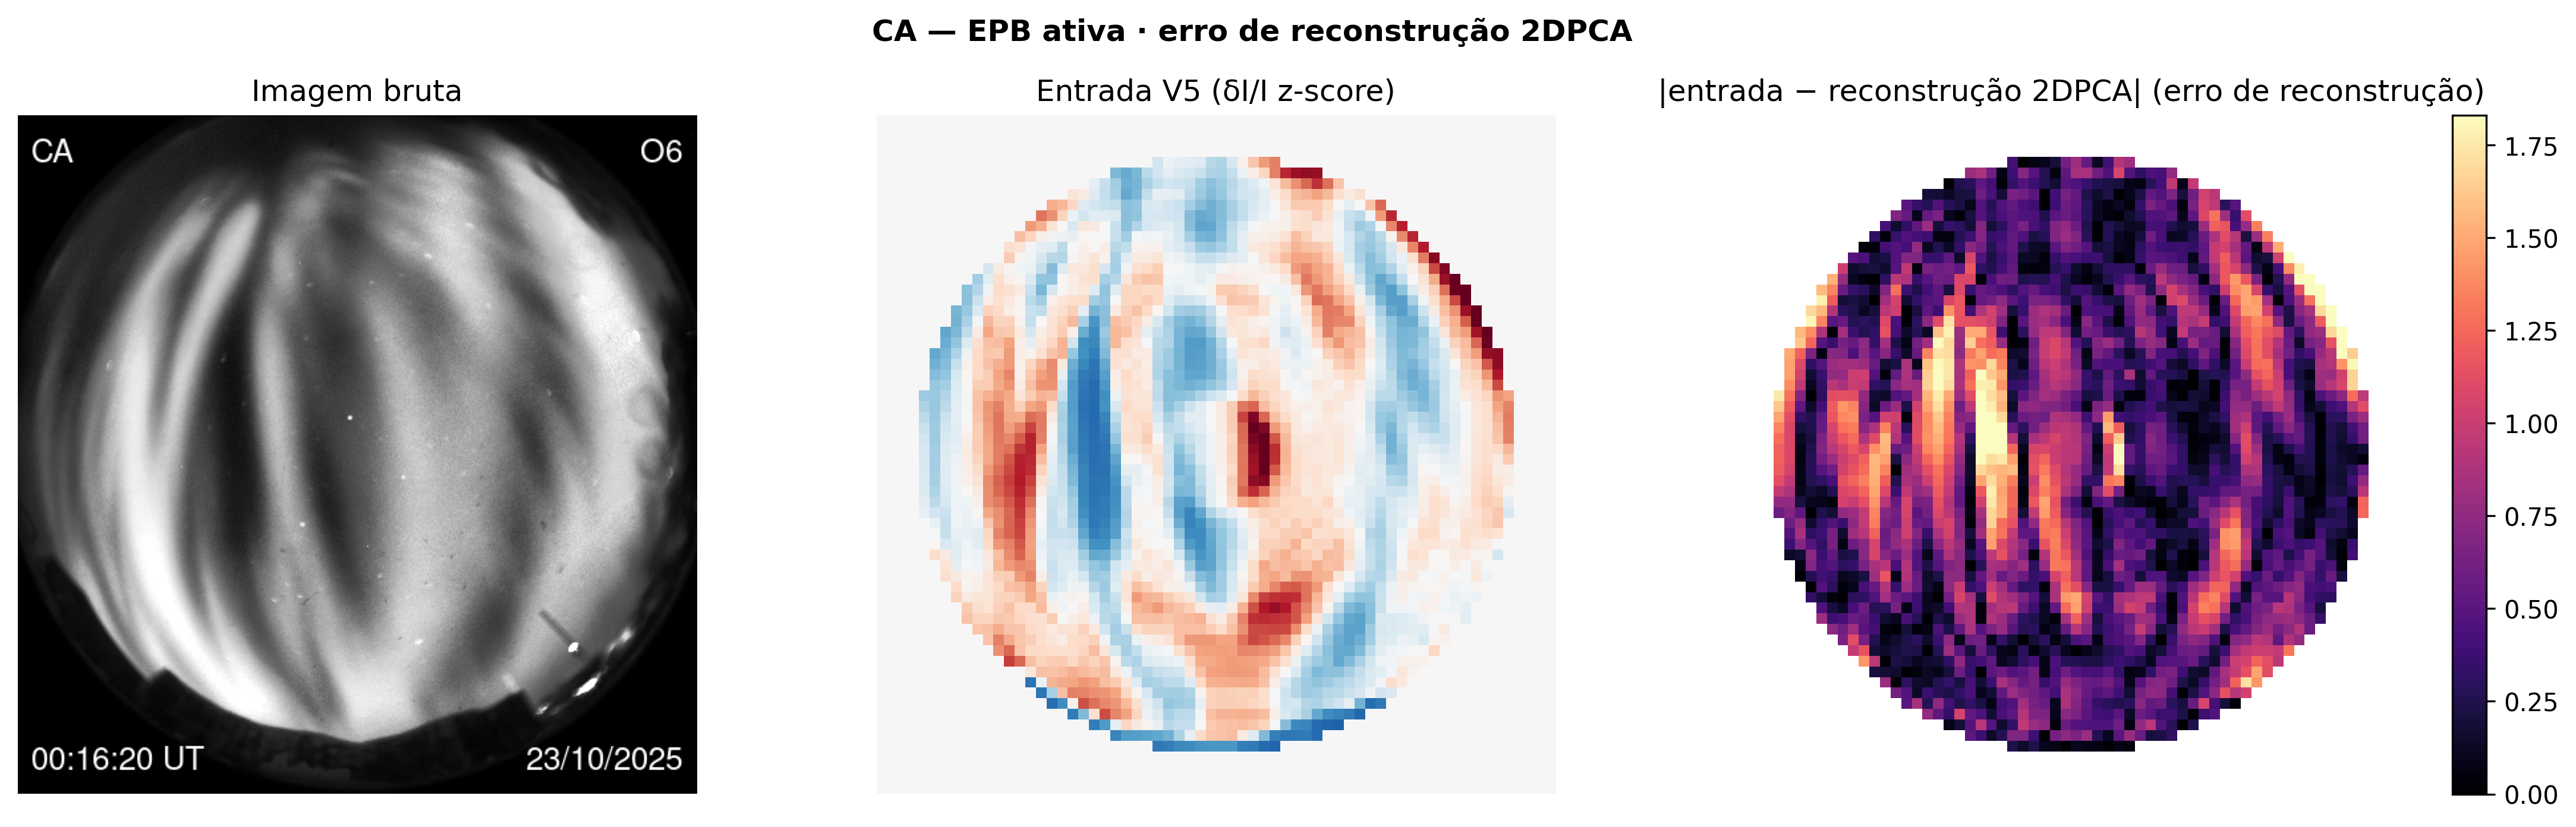
\includegraphics[width=0.96\textwidth]{figs/recon_error_with.png}
    \caption{Unsupervised 2DPCA subspace reconstruction analysis for an active EPB exposure (predicted EPB probability $99.2\%$). Large reconstruction residuals trace the North-South plasma depletion bands.}
    \label{fig:recon_error_with}
\end{figure}

Figures~\ref{fig:recon_error_without} and~\ref{fig:recon_error_with} show the $k=5$ reconstruction for a quiet and an active frame. In the quiet frame from BJL, the error is low inside the dome and appears only at the lens border and along a faint Milky Way streak. In the active frame from CA, the dark, bifurcated depletions create sharp intensity transitions, and the error exceeds $0.4$ along the whole north--south length of the bubbles.

\subsection{Cross-Validation Across Splitting Protocols}

Table~\ref{tab:cv_protocols} summarizes the results under each validation protocol. In stratified cross-validation (Figure~\ref{fig:kfold_cv}), the ensemble reached $97.20\%$ accuracy and $96.78\%$ F1-score, with specificity ($98.74\%$) higher than sensitivity ($95.30\%$); the PR-AUC was $0.9980 \pm 0.0018$. Pooling the out-of-fold predictions of all $572$ images (Figures~\ref{fig:confusion_matrix} and~\ref{fig:roc_pr}) gives only $4$ false positives against $12$ false negatives, so most errors are missed bubbles rather than false alarms. The holdout split ($64$ EPB and $79$ non-EPB images) gave similar numbers, with $96.50\%$ accuracy and a negative predictive value of $96.25\%$.

\begin{table}[htbp]
\centering
\caption{Performance of the 2DPCA ($k=5$) + Stacking Ensemble across validation protocols on the labeled dataset ($N=572$, mean $\pm$ standard deviation across folds).}
\label{tab:cv_protocols}
\resizebox{\textwidth}{!}{%
\setlength{\tabcolsep}{4pt}
\begin{tabular}{lcccccc}
\toprule
\textbf{Validation Protocol} & \textbf{Acc (\%)} & \textbf{Sens (\%)} & \textbf{Spec (\%)} & \textbf{Prec (\%)} & \textbf{F1 (\%)} & \textbf{ROC-AUC} \\
\midrule
5-Fold Stratified CV ($N=572$) & $97.20 \pm 1.57$ & $95.30 \pm 4.51$ & $98.74 \pm 1.32$ & $98.45 \pm 1.59$ & $96.78 \pm 1.86$ & $0.9984 \pm 0.0016$ \\
5-Fold Temporal-Block CV ($77$ blocks) & $95.08 \pm 5.72$ & $90.88 \pm 10.48$ & $98.79 \pm 2.71$ & $98.60 \pm 3.14$ & $94.24 \pm 5.37$ & $0.9969 \pm 0.0066$ \\
5-Fold Circular FOV Mask CV ($N=572$) & $95.80 \pm 1.57$ & $93.34 \pm 4.72$ & $97.79 \pm 1.80$ & $97.24 \pm 2.15$ & $95.16 \pm 1.89$ & $0.9976 \pm 0.0011$ \\
Holdout Test Split ($n=143$) & $96.50$ & $95.31$ & $97.47$ & $96.83$ & $96.06$ & $0.9974$ \\
\bottomrule
\end{tabular}%
}
\end{table}

\begin{figure}[htbp]
    \centering
    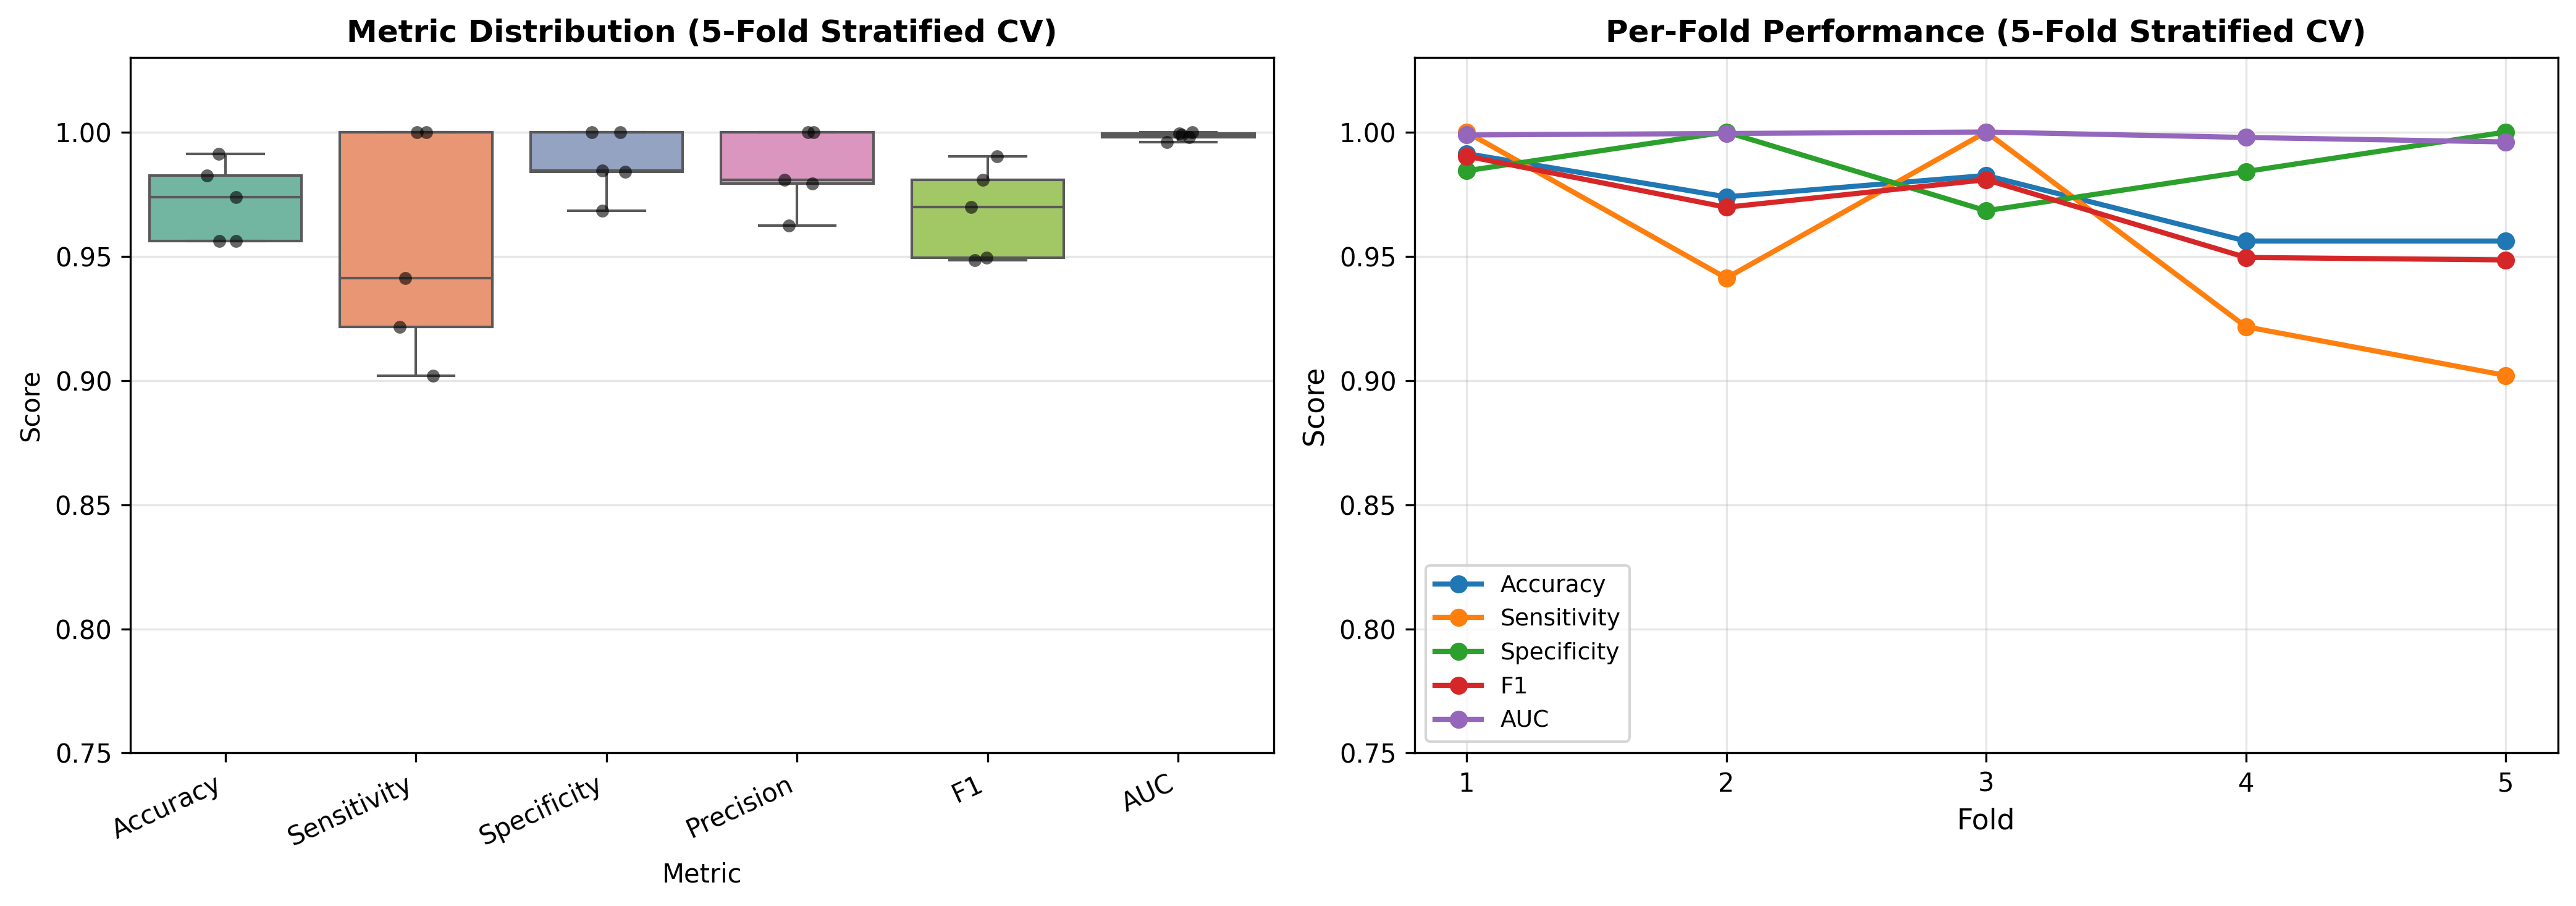
\includegraphics[width=0.98\textwidth]{figs/kfold_cv_metrics.png}
    \caption{Left: Boxplot distribution of classification metrics across the 5 stratified folds ($N=572$). Right: Per-fold metric trajectories.}
    \label{fig:kfold_cv}
\end{figure}

\begin{figure}[htbp]
    \centering
    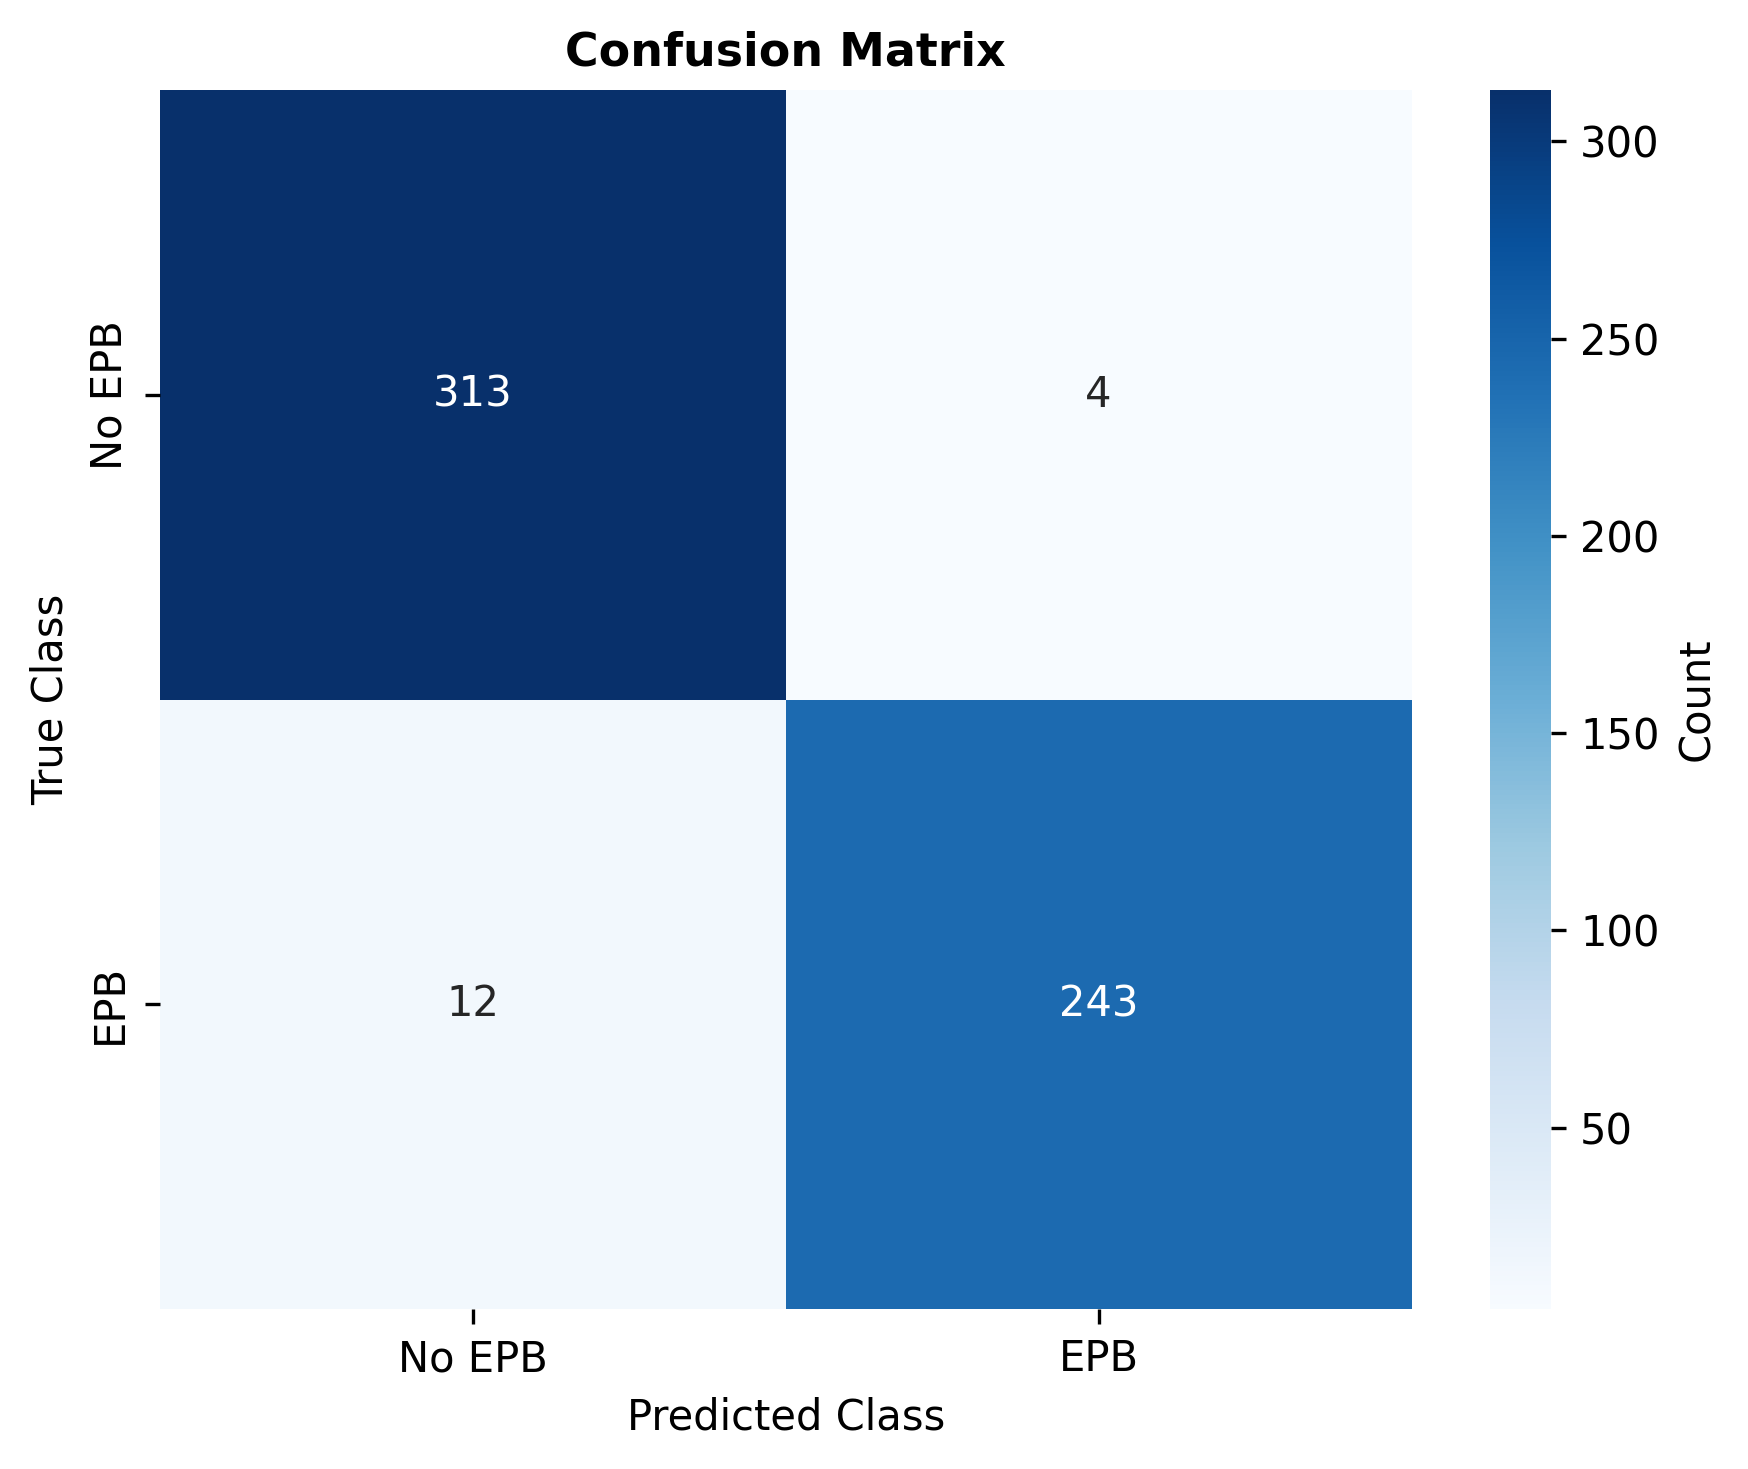
\includegraphics[width=0.52\textwidth]{figs/confusion_matrix.png}
    \caption{Out-of-fold confusion matrix aggregated across all $N=572$ labeled exposures ($313$ TN, $4$ FP, $12$ FN, $243$ TP).}
    \label{fig:confusion_matrix}
\end{figure}

\begin{figure}[htbp]
    \centering
    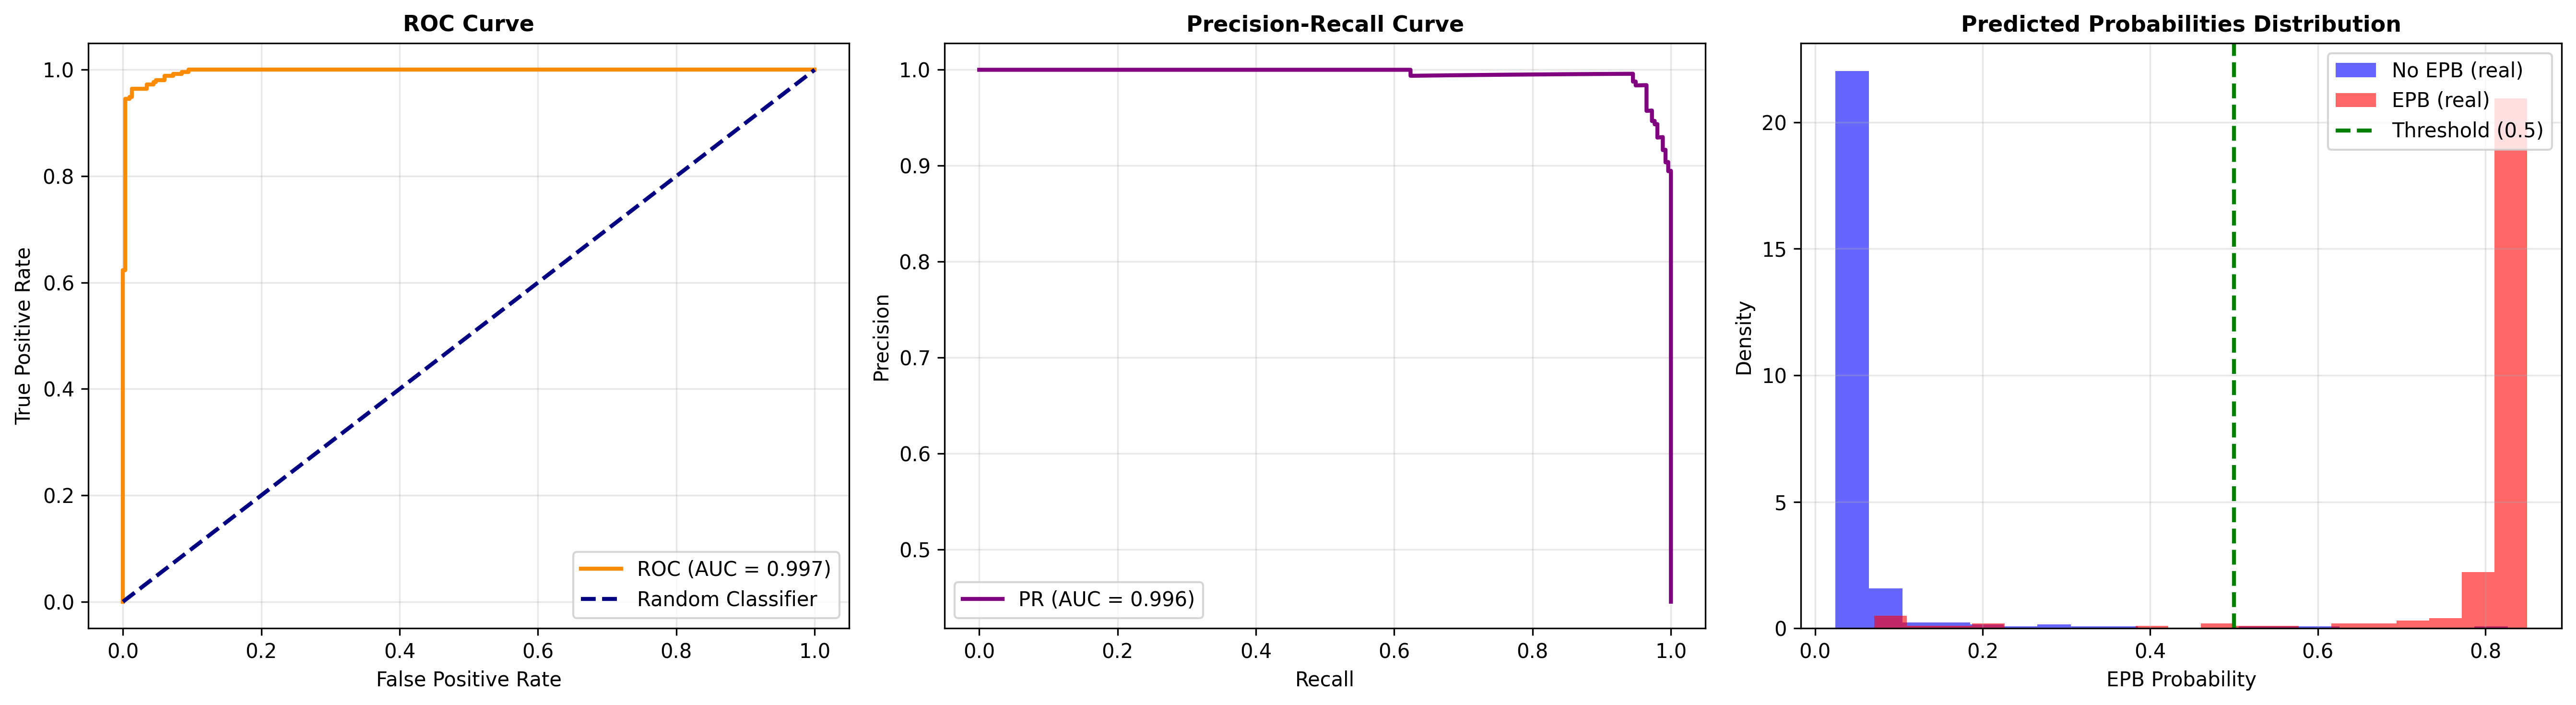
\includegraphics[width=0.98\textwidth]{figs/roc_pr_curves.png}
    \caption{Aggregated out-of-fold ROC curve (AUC $= 0.997$), Precision-Recall curve (AUC $= 0.996$), and predicted probability histogram across all $N=572$ labeled images.}
    \label{fig:roc_pr}
\end{figure}

Keeping each $30$-minute window inside a single fold lowered accuracy to $95.08\%$ and, above all, made sensitivity vary much more between folds ($90.88\% \pm 10.48\%$). This is expected: when a whole active window is held out, some depletion shapes are missing from training. ROC-AUC, however, stayed at $0.9969$ (PR-AUC $0.9978$), so the separation between classes does not depend on near-identical frames shared by training and validation. With the circular mask that hides the corner text, accuracy was $95.80\%$, about $1.4$ points below the unmasked model, and the holdout accuracy was unchanged ($96.50\%$). The classifier, therefore, does not rely on the printed annotations.

\subsection{Baselines, Ablations, and Shortcut Learning}

Table~\ref{tab:benchmark} and Figure~\ref{fig:benchmark} compare the pipeline with the baselines and ablations described in Section~\ref{sec:protocol}. Besides the holdout metrics, the table gives the zero-shot recall on CP (ZS-CP), which shows whether a good holdout score comes from the EPB structure or from cues tied to the station.

\begin{table}[htbp]
\centering
\caption{Baseline and ablation comparison on the stratified holdout test set ($n=143$), zero-shot recall on the unseen Cachoeira Paulista observatory (ZS-CP, $n=42$), and single-frame CPU inference latency.}
\label{tab:benchmark}
\resizebox{\textwidth}{!}{%
\setlength{\tabcolsep}{4pt}
\begin{tabular}{lcccccccc}
\toprule
\textbf{Model / Ablation Configuration} & \textbf{Acc} & \textbf{Sens} & \textbf{Spec} & \textbf{Prec} & \textbf{F1} & \textbf{ROC-AUC} & \textbf{ZS-CP} & \textbf{ms/img} \\
\midrule
Flatten ($4096$) + Logistic Regression & 0.9790 & 0.9688 & 0.9873 & 0.9841 & 0.9764 & 0.9992 & 0.9762 & 0.050 \\
1D-PCA ($320$) + Logistic Regression & 0.9860 & 1.0000 & 0.9747 & 0.9697 & 0.9846 & 0.9994 & 0.6905 & 0.070 \\
1D-PCA ($320$) + SVM (RBF) & 0.9510 & 1.0000 & 0.9114 & 0.9014 & 0.9481 & 0.9921 & 1.0000 & 0.231 \\
Flatten ($4096$) + Random Forest & 0.9720 & 1.0000 & 0.9494 & 0.9412 & 0.9697 & 0.9996 & 0.5476 & 0.678 \\
2DPCA ($k=5$) + SVM (RBF) & 0.9650 & 0.9688 & 0.9620 & 0.9538 & 0.9612 & 0.9978 & 1.0000 & 0.087 \\
2DPCA ($k=5$) + Random Forest & 0.9371 & 0.9062 & 0.9620 & 0.9508 & 0.9280 & 0.9909 & 1.0000 & 0.749 \\
2DPCA ($k=5$) + XGBoost & 0.9510 & 0.9375 & 0.9620 & 0.9524 & 0.9449 & 0.9958 & 1.0000 & 0.027 \\
2D-CNN (ConvNet Baseline) & 0.9720 & 1.0000 & 0.9494 & 0.9412 & 0.9697 & 0.9974 & 1.0000 & 0.769 \\
\midrule
Ablation: No Radiometric Preprocessing & 0.9930 & 1.0000 & 0.9873 & 0.9846 & 0.9922 & 1.0000 & 0.0000 & 0.570 \\
Ablation: No SMOTE Balancing & 0.9650 & 0.9531 & 0.9747 & 0.9683 & 0.9606 & 0.9970 & 1.0000 & 0.621 \\
Ablation: Circular FOV Mask & 0.9650 & 0.9531 & 0.9747 & 0.9683 & 0.9606 & 0.9964 & 1.0000 & 0.456 \\
2DPCA + Stacking Ensemble (Proposed) & 0.9650 & 0.9531 & 0.9747 & 0.9683 & 0.9606 & 0.9974 & 1.0000 & 0.630 \\
\bottomrule
\end{tabular}%
}
\end{table}

\begin{figure}[htbp]
    \centering
    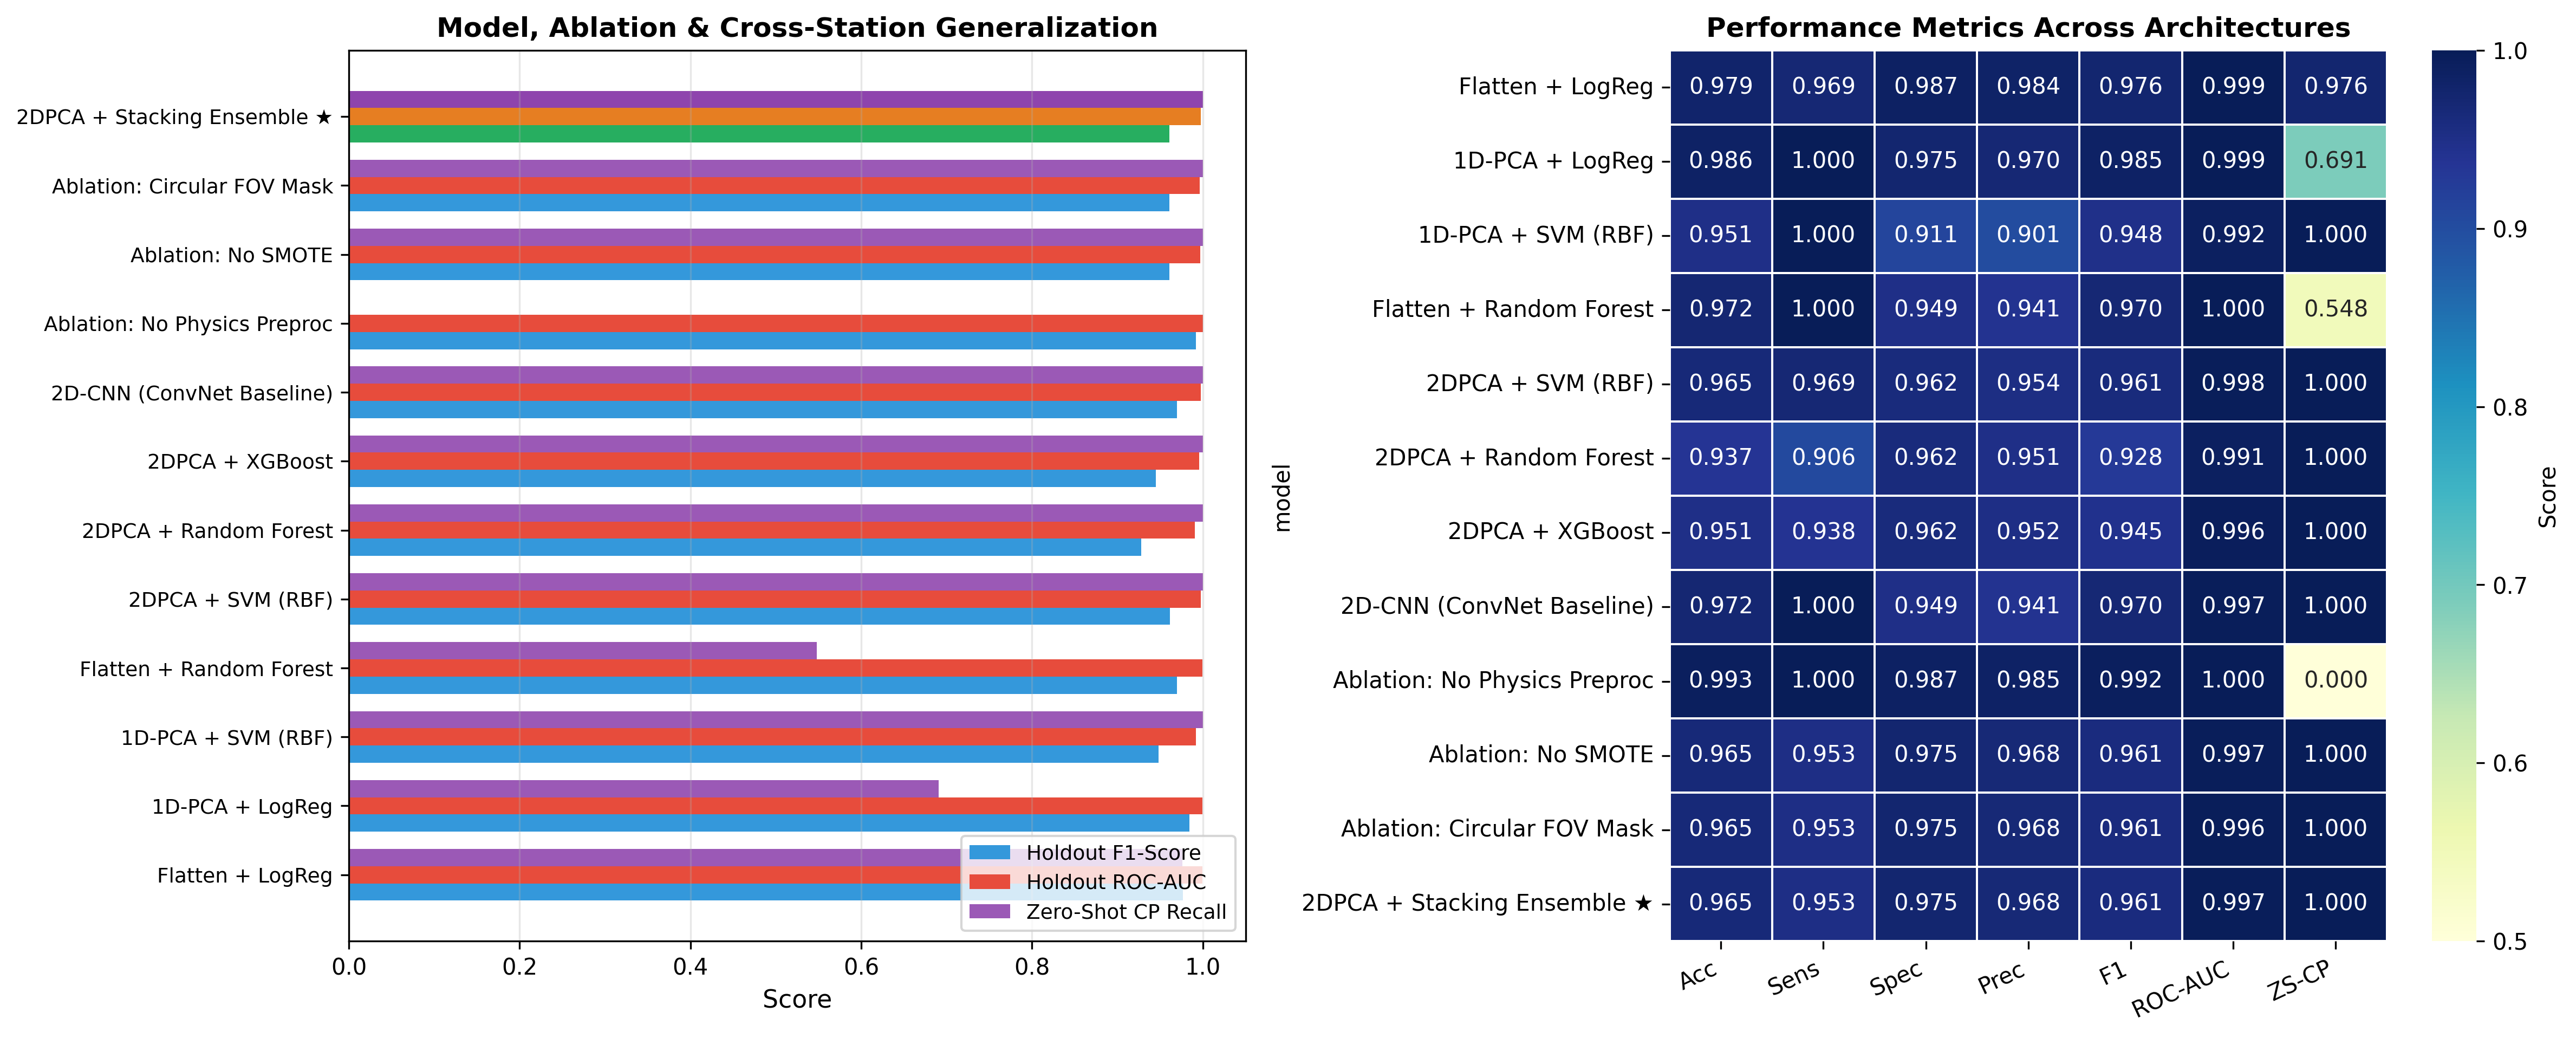
\includegraphics[width=0.98\textwidth]{figs/benchmark_baselines.png}
    \caption{Comparison of holdout F1-score, holdout ROC-AUC, and zero-shot Cachoeira Paulista recall (ZS-CP) across baselines, individual 2DPCA learners, 2D-CNN, and ablations.}
    \label{fig:benchmark}
\end{figure}

On the holdout split, the model without radiometric preprocessing had the best accuracy ($0.9930$), and the flattened and 1D-PCA models reached $0.9510$--$0.9860$. On CP, however, the model without preprocessing did not detect a single EPB ($0/42$). The most likely explanation is that, without background subtraction and CLAHE, it separated BJL (only negatives) from CA (mostly positives) by their overall brightness, a cue that does not hold at CP, whose background is brighter. Flatten + Random Forest and 1D-PCA + Logistic Regression also lost much of their recall at CP ($54.76\%$, $23/42$, and $69.05\%$, $29/42$), probably because they give weight to pixel positions tied to the geometry of each camera.

All models built on preprocessed 2DPCA features detected the $42$ EPB frames at CP, as did the 2D CNN and 1D-PCA + SVM. Within this group, the stacking ensemble had the highest specificity ($97.47\%$, against $96.20\%$ for each 2DPCA learner alone and $94.94\%$ for the CNN), with an inference time of $0.63\text{ ms}$ per image. Removing SMOTE did not change holdout accuracy ($0.9650$), which is expected given the mild $1.24:1$ class ratio, but it lowered the mean predicted probability on CP from $75.71\%$ to $68.50\%$. In-fold SMOTE thus makes the model more confident on the unseen station.

\subsection{Moonlight, Station Effects, and Cloud Screening}

Table~\ref{tab:hard_negatives} groups the operational tests. When the out-of-fold predictions are split by Moon illumination, accuracy is $97.47\%$ for images taken with less than $50\%$ illumination. On the $97$ bright-moon images (up to $99.6\%$ illumination), where glare saturates part of the dome, specificity is $95.88\%$: only four of these hard negatives were taken for EPBs, which suggests that the background subtraction removes most of the smooth glare gradient. By station, out-of-fold accuracy is $94.84\%$ at CA, which includes clear and partly cloudy periods, and $100\%$ at BJL and CP.

The full-night sequences show why Stage~1 is needed. Used alone, the Stage~2 classifier trained on clear skies raised a false alarm on $61$ of the $62$ frames of the overcast night \texttt{CA\_20260624}, because CLAHE turns dark cloud edges into high-contrast bands. With Stage~1, $49$ frames ($79.0\%$) were labeled \texttt{CLOUDY} and $7$ ($11.3\%$) \texttt{DEGRADED}, and false alarms fell from $61$ to $13$ ($-78.7\%$), or to $6$ ($-90.2\%$) if alerts are issued only for \texttt{CLEAR} frames. On the clear night \texttt{BJL\_20250722}, Stage~1 blocked $14$ twilight or hazy frames ($6.1\%$) and, with them, the $3$ false alarms produced by Stage~2 alone. On the active night \texttt{CA\_20251022}, only $4$ frames ($2.9\%$) were flagged as cloudy, and $125$ EPB detections were kept ($89.3\%$ of the frames, $122$ of them under \texttt{CLEAR} sky).

\begin{table}[htbp]
\centering
\caption{Operational evaluation across lunar illumination regimes, observatory sites (including zero-shot transfer to CP), and continuous nocturnal sequences comparing Stage~2 alone (trained on clear skies, $n=510$) against the two-stage cascaded pipeline.}
\label{tab:hard_negatives}
\resizebox{\textwidth}{!}{%
\setlength{\tabcolsep}{4.5pt}
\begin{tabular}{llcccc}
\toprule
\textbf{Evaluation Scenario} & \textbf{Protocol / Mode} & \textbf{Frames} & \textbf{QC Flagged} & \textbf{Metric / Result} \\
\midrule
Low/Moderate Moon ($<50\%$) & 5-Fold OOF & 475 & -- & Acc: $97.47\%$ / Spec: $100.0\%$ ($220/220$) \\
Bright Lunar Glare ($\ge 50\%$) & 5-Fold OOF (Hard Neg.) & 97 & -- & Specificity: $95.88\%$ ($93/97$) \\
\midrule
São João do Cariri (CA) & 5-Fold OOF & 310 & -- & Accuracy: $94.84\%$ \\
Bom Jesus da Lapa (BJL) & 5-Fold OOF & 220 & -- & Specificity: $100.0\%$ ($220/220$) \\
Cachoeira Paulista (CP) & Zero-Shot (Train: CA+BJL) & 42 & -- & Recall: $100.0\%$ ($42/42$) \\
\midrule
\texttt{BJL\_20250722} (Clear Quiet) & Stage 2 Only vs. Cascaded & 230 & $14$ ($6.1\%$) & FP: $3 \to 0$ ($100.0\%$ Spec.) \\
\texttt{CA\_20260624} (Overcast Sky) & Stage 2 Only vs. Cascaded & 62 & $49$ ($79.0\%$) & FP: $61 \to 13$ ($6$ Clear, $-78.7\%$ / $-90.2\%$) \\
\texttt{CA\_20251022} (Active EPB) & Stage 2 Only vs. Cascaded & 140 & $4$ ($2.9\%$) & Valid EPB: $125$ ($89.3\%$) \\
\bottomrule
\end{tabular}%
}
\end{table}

\subsection{SHAP Attribution and Full-Night Time Series}

Figures~\ref{fig:shap_without} and~\ref{fig:shap_with} show the SHAP values mapped back to pixel space (Section~\ref{sec:model}) for the same quiet and active frames used in Figures~\ref{fig:recon_error_without} and~\ref{fig:recon_error_with}.

\begin{figure}[htbp]
    \centering
    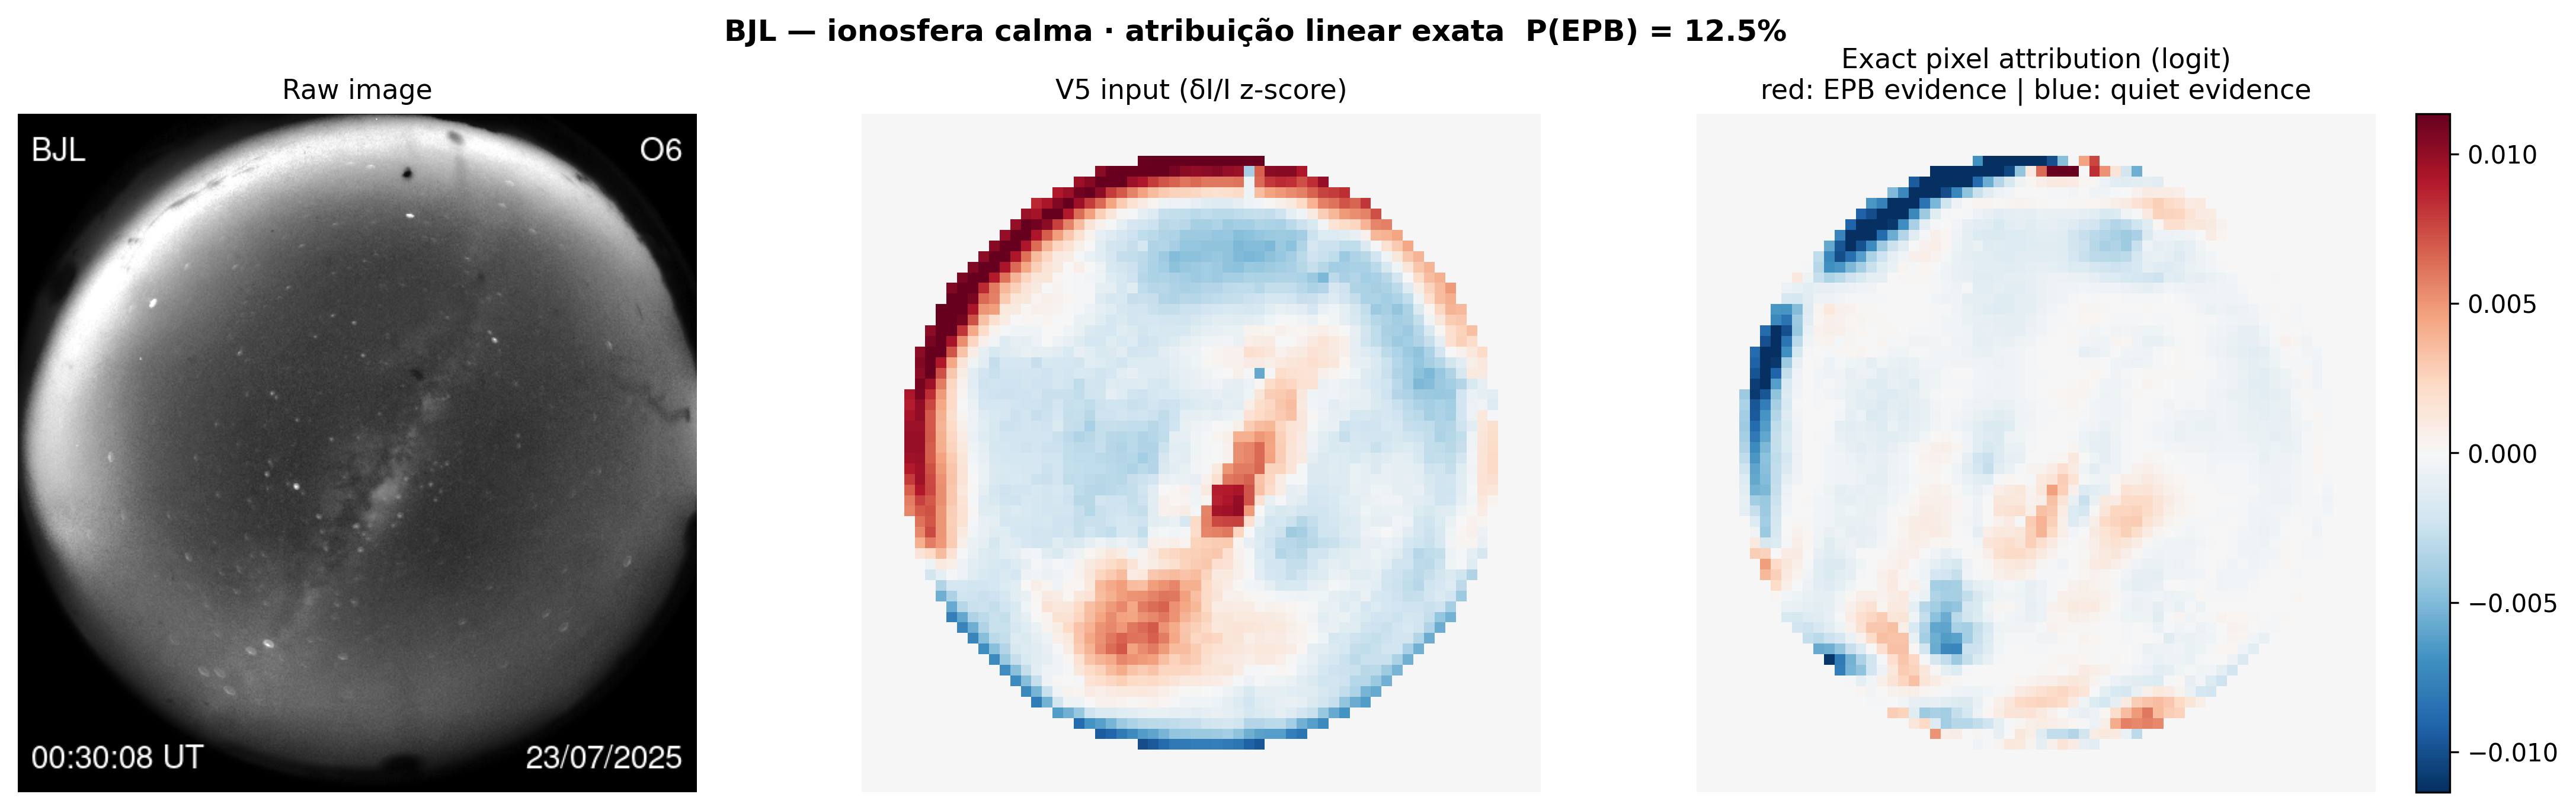
\includegraphics[width=0.98\textwidth]{figs/shap_analysis_without.png}
    \caption{Pixel-space SHAP attribution for a quiet-sky exposure from Bom Jesus da Lapa (True: No EPB, Predicted: No EPB, $0.4\%$). Blue regions denote negative attributions that reduce EPB probability.}
    \label{fig:shap_without}
\end{figure}

\begin{figure}[htbp]
    \centering
    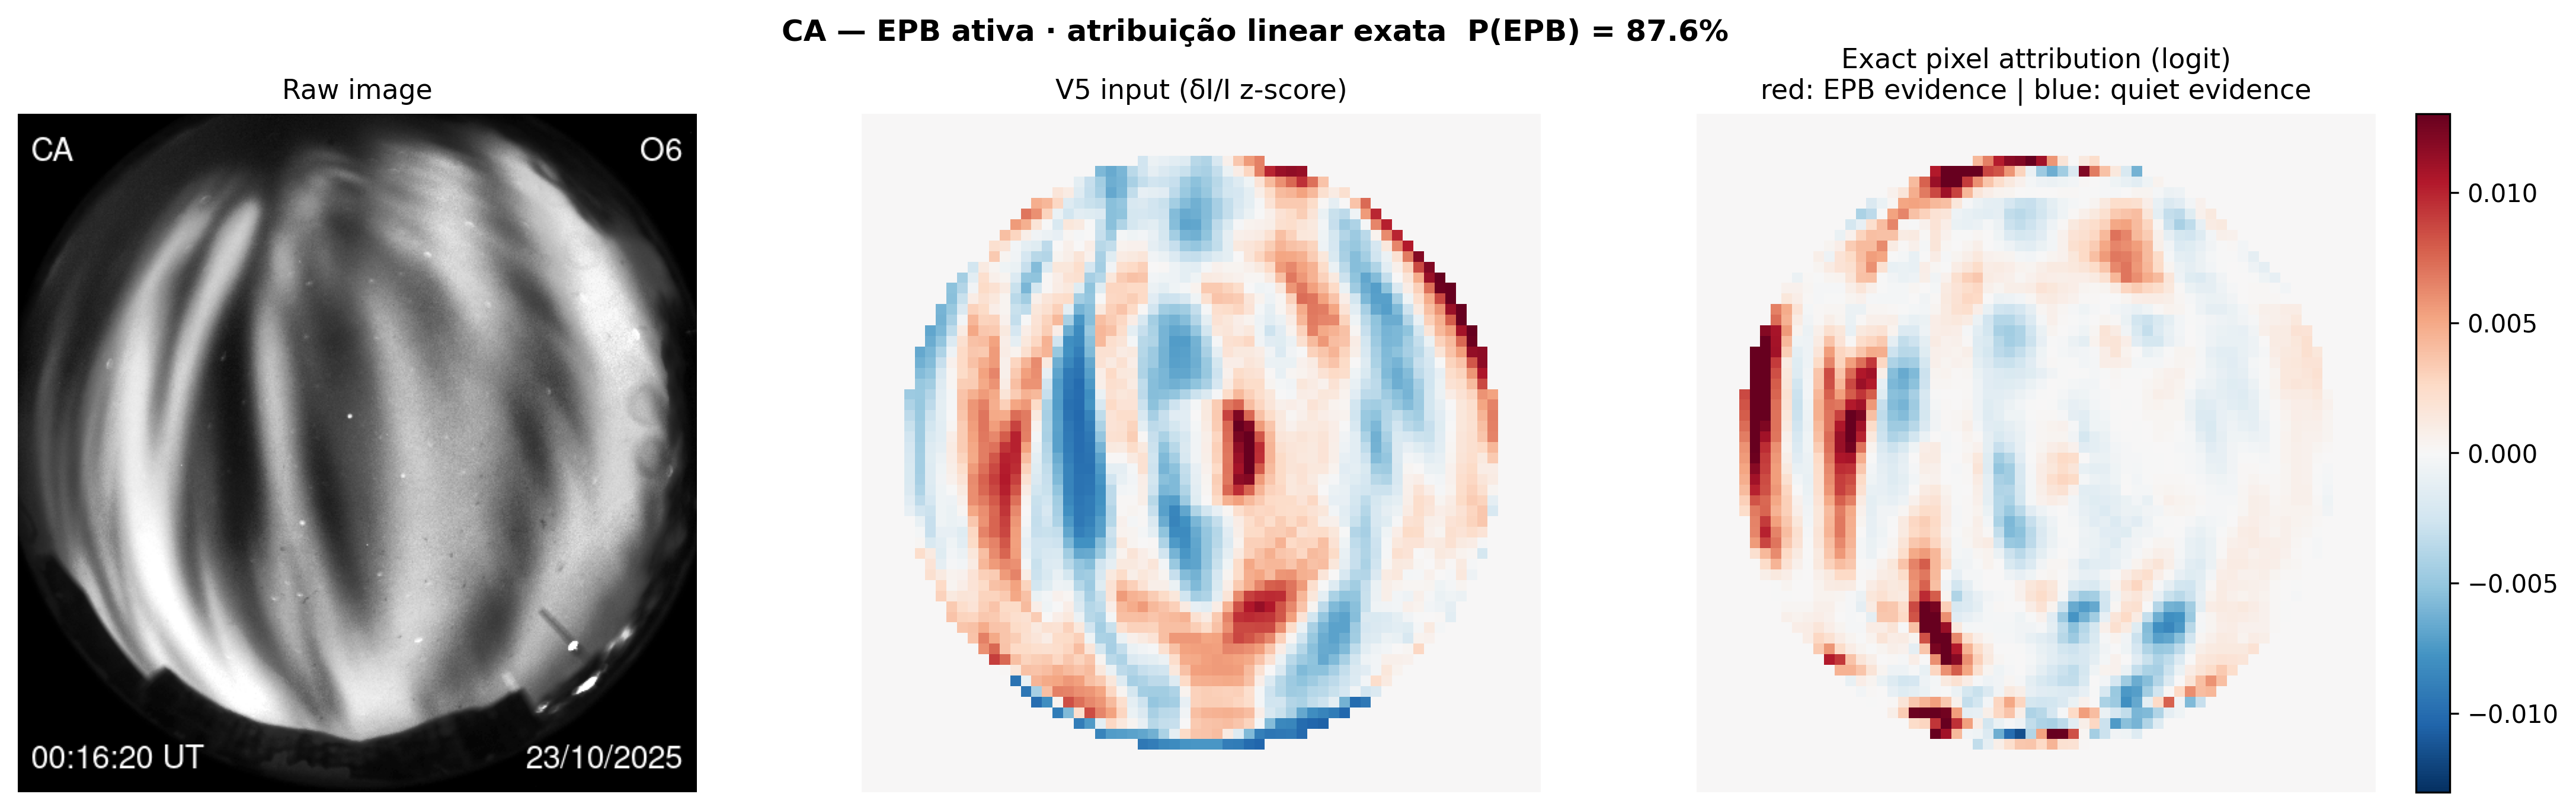
\includegraphics[width=0.98\textwidth]{figs/shap_analysis_with.png}
    \caption{Pixel-space SHAP attribution for an active EPB exposure from Cariri (True: EPB, Predicted: EPB, $99.2\%$). Red bands mark positive attributions aligned with the plasma depletion channels.}
    \label{fig:shap_with}
\end{figure}

In the quiet frame, negative values cover the center of the dome and keep the EPB probability at $0.4\%$. In the active frame ($99.2\%$), positive values follow the dark north--south depletion bands, and the four corners with text receive almost no attribution.

\begin{figure}[htbp]
    \centering
    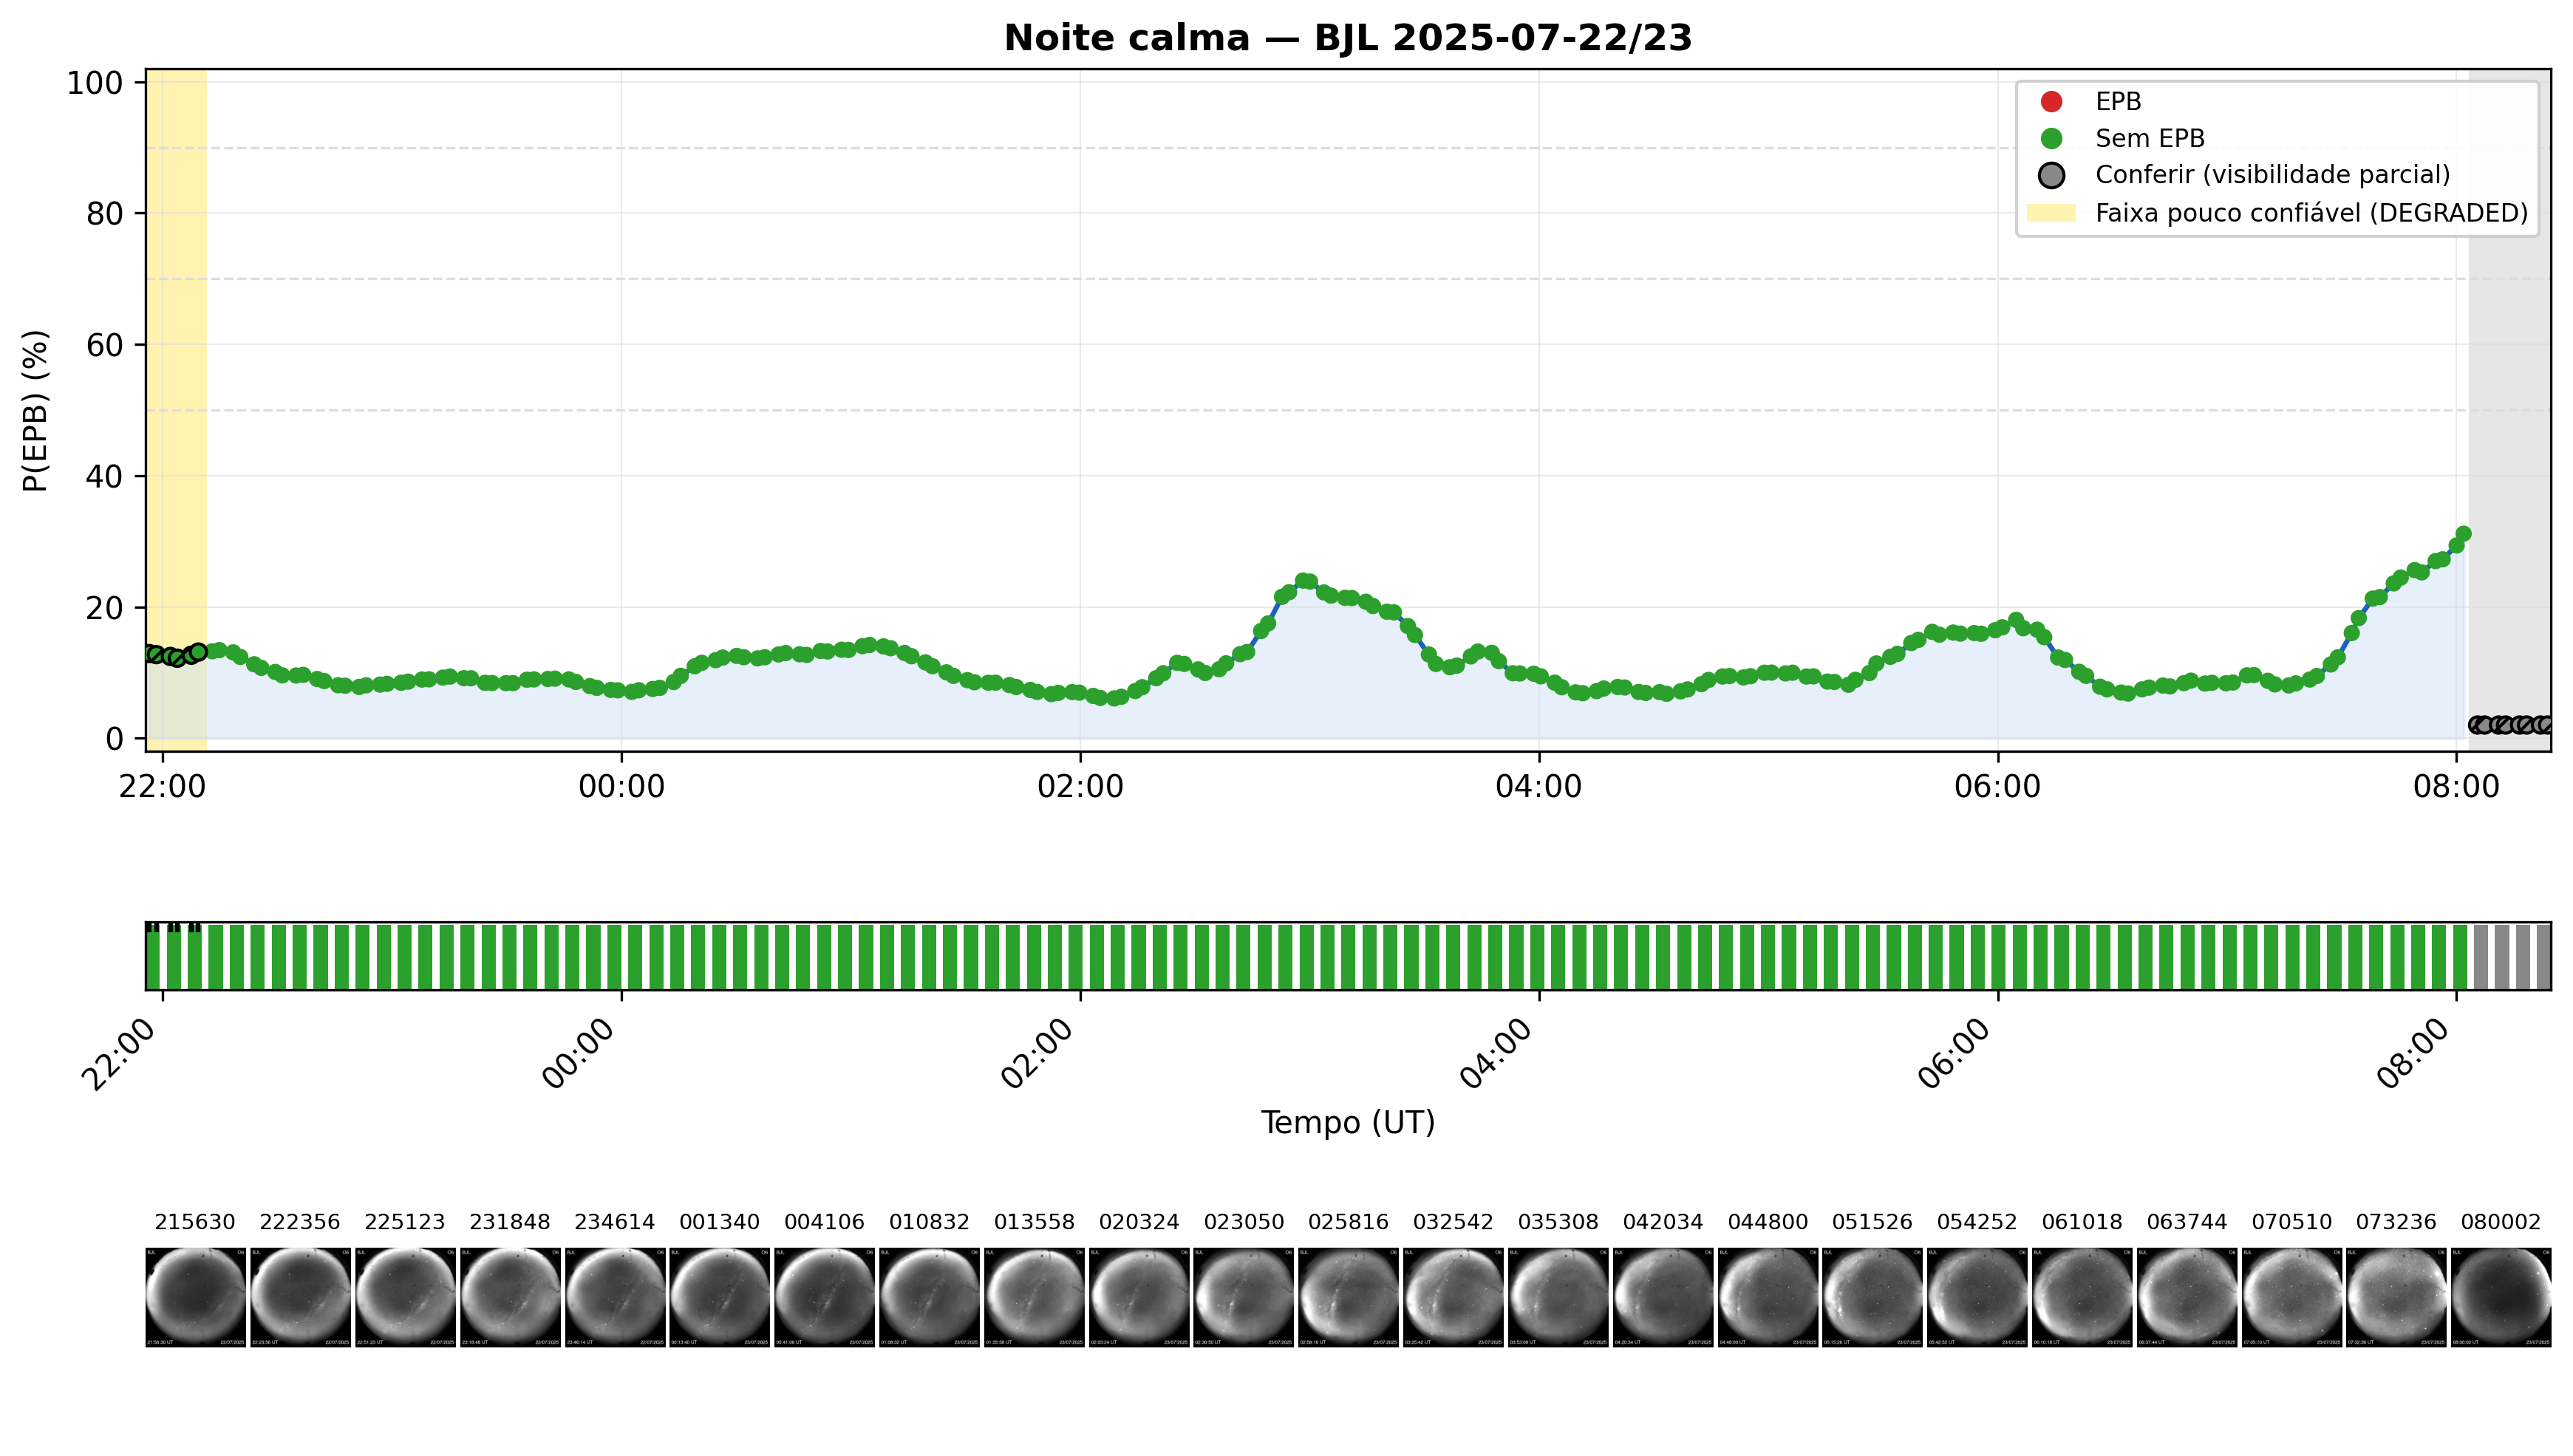
\includegraphics[width=0.98\textwidth]{figs/temporal_without_epb.png}
    \caption{Nocturnal time series on a clear quiet night at Bom Jesus da Lapa (\texttt{BJL\_20250722}, $230$ exposures). Predicted EPB probabilities remain near $0.4\%$ all night ($0$ false alarms).}
    \label{fig:temporal_without}
\end{figure}

\begin{figure}[htbp]
    \centering
    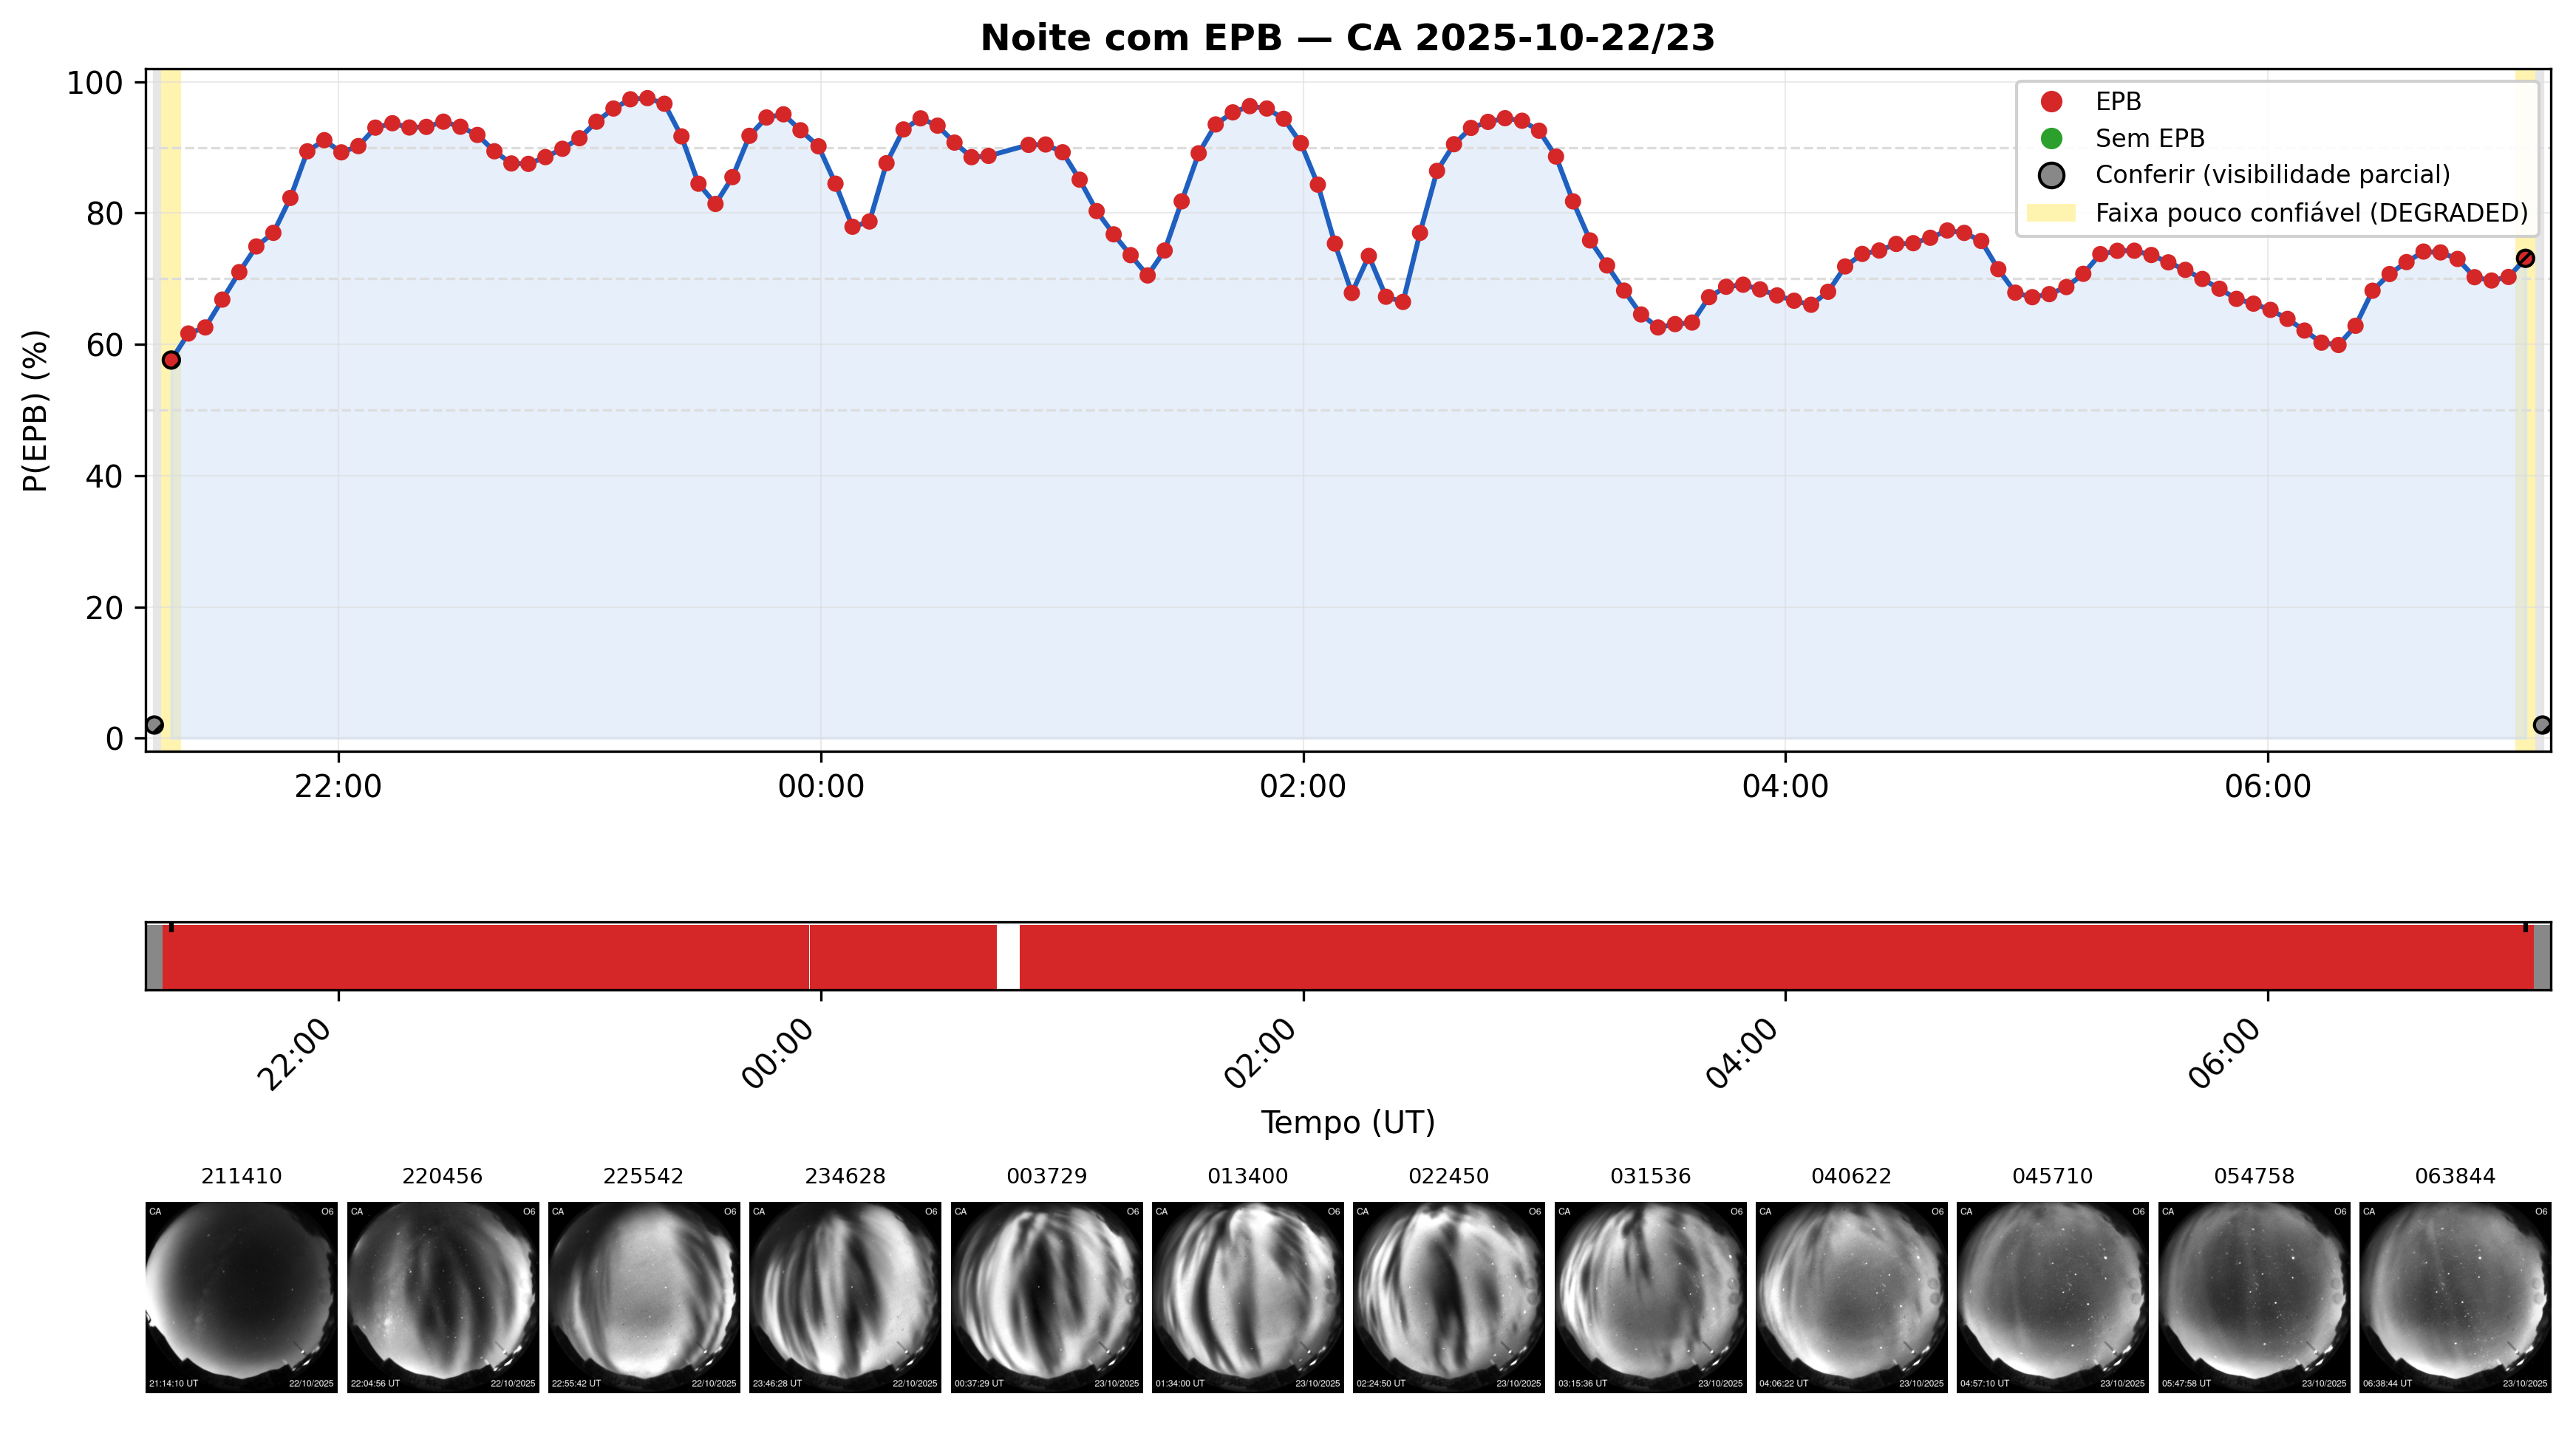
\includegraphics[width=0.98\textwidth]{figs/temporal_with_epb.png}
    \caption{Nocturnal time series on an active EPB night at Cariri (\texttt{CA\_20251022}, $140$ exposures), capturing bubble onset after $21{:}18\text{ UT}$, sustained zenith passage ($138/140$ frames), and pre-dawn decay.}
    \label{fig:temporal_with}
\end{figure}

\begin{figure}[htbp]
    \centering
    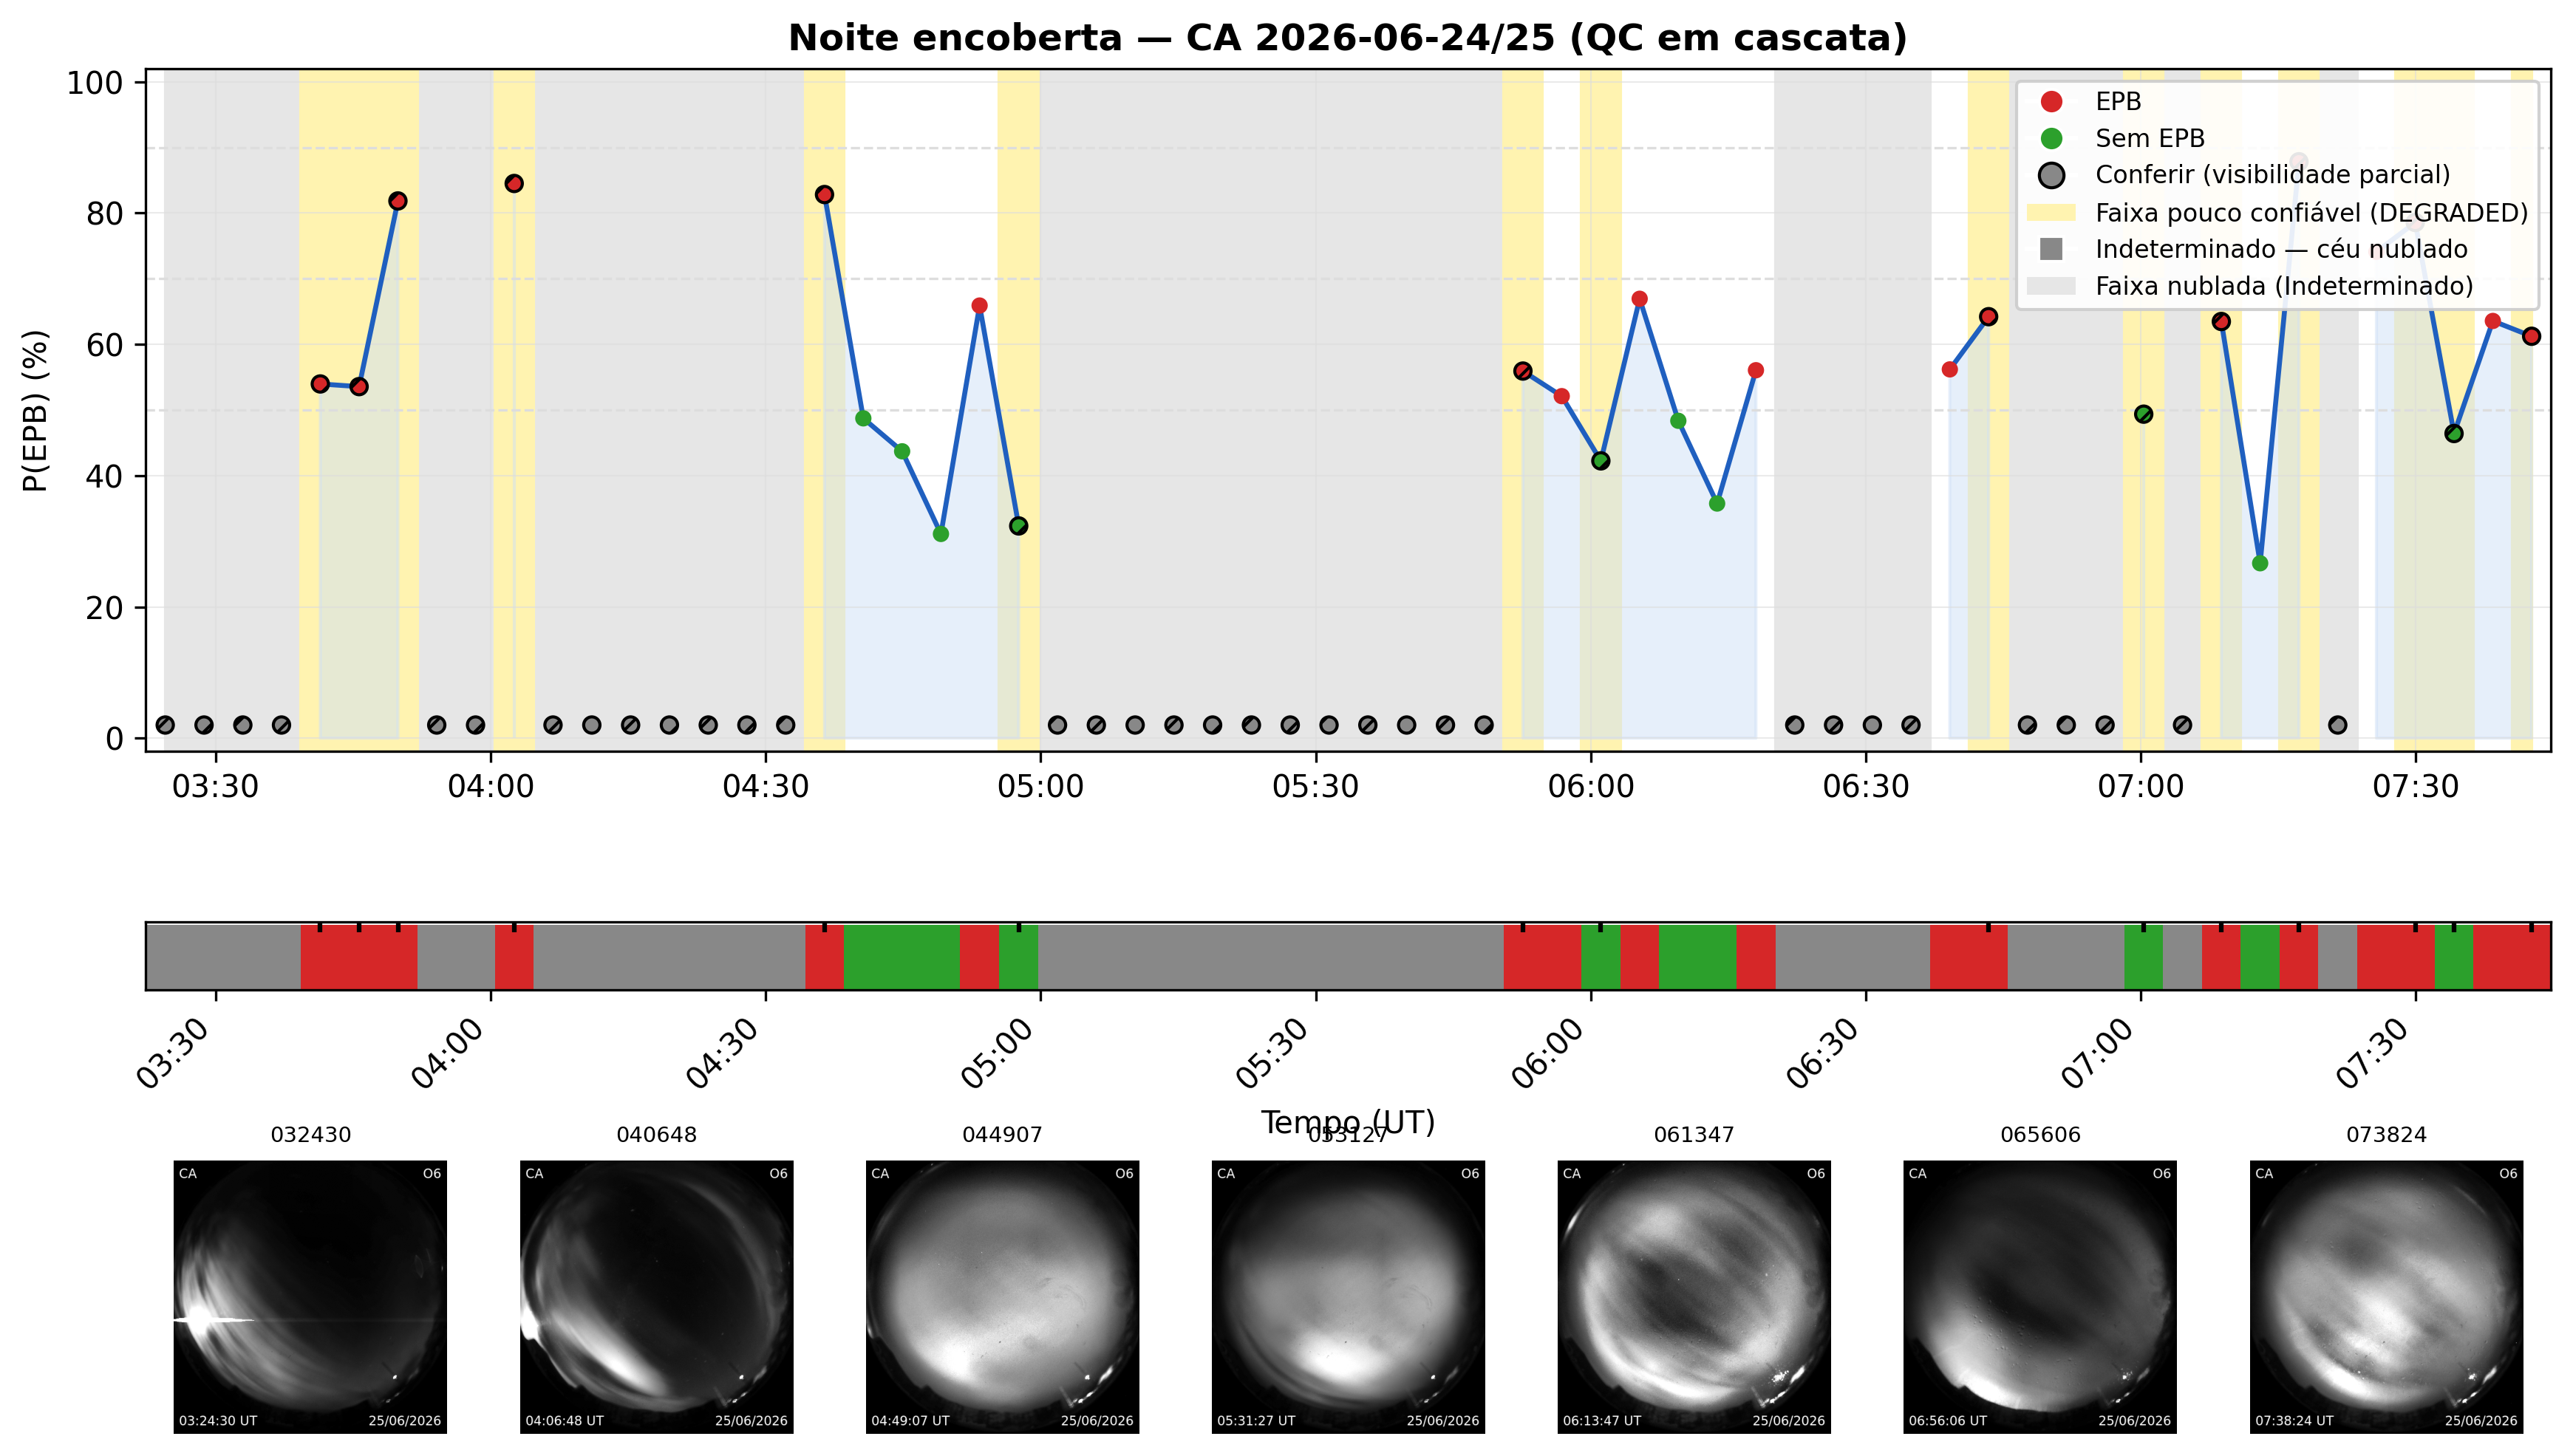
\includegraphics[width=0.98\textwidth]{figs/temporal_cloudy_qc.png}
    \caption{Cascaded nocturnal monitoring on an overcast night at Cariri (\texttt{CA\_20260624}, $62$ exposures). Stage~1 Sky QC (gray status intervals) flags $49/62$ frames ($79.0\%$) as cloudy.}
    \label{fig:temporal_cloudy}
\end{figure}

Figures~\ref{fig:temporal_without}--\ref{fig:temporal_cloudy} show the output of the final model over complete nights. On the quiet night \texttt{BJL\_20250722}, the probability stays around $0.4\%$ for all $230$ frames. On the active night \texttt{CA\_20251022}, it crosses the decision threshold at $21{:}18$~UT ($63.8\%$), reaches $99\%$ when the bubbles pass the zenith, stays high for the rest of the night (mean of $92.0\%$ over $138$ of the $140$ frames), and drops to $2.1\%$ at $07{:}08$~UT, as the depletions fade before dawn. On the overcast night \texttt{CA\_20260624}, Stage~1 masks most of the night and leaves only short clear intervals to be classified.
